\documentclass[10pt,openright,twoside,french]{book}

\input philippe2013
\input philippe2013_cours
\input philippe2013_sections
\input philippe2013_chapitre

\usepackage{docmute}

\begin{document}

%___________________________
%===    Page de garde
%------------------------------------------------------

\frontmatter

\titlepage{
\begin{center}
{\Large\bfseries\color{midblue} Philippe \bsc{De Sousa}}

\vspace*{\stretch{1}}

\begin{tikzpicture}[scale=1.5]
\begin{scope}
% style des noeuds
\tikzstyle{debutfin}=[ellipse,draw,text=red]
\tikzstyle{instruct}=[rectangle,draw,fill=yellow!50]
\tikzstyle{test}=[diamond, aspect=2.5,thick,draw=blue,fill=yellow!50,text=blue]
\tikzstyle{es}=[rectangle,draw,rounded corners=4pt,fill=blue!25]
% style des flèches
\tikzstyle{suite}=[->,>=stealth',thick,rounded corners=4pt]
% placement des noeuds
\node[debutfin] (debut) at (-3,11) {Début};
\node[es] (lire) at (-3,9) {\begin{tabular}{c}Lire un entier positif $A$ \\ Lire un entier positif $B$\end{tabular}};
\node[instruct] (init) at (-3,6) {\begin{tabular}{c}$Q\leftarrow ENT(A \div B)$ \\ $R\leftarrow A - B \times Q$\end{tabular}};
\node[test] (test) at (-3,4) {$R = 0$ \ ?};
\node[es] (affichage) at (-3,1) {$PGCD = B$};
\node[debutfin] (fin) at (-3,-1) {Fin};
\node[es] (remplace) at (1,6) {\begin{tabular}{c}$A\leftarrow B$ \\ $B\leftarrow R$\end{tabular}};
% Placement des flèches
\draw[suite] (debut) -- (lire);
\draw[suite] (lire) -- (init);
\draw[suite] (init) -- (test.north);
\draw[suite] (test) -- (affichage) node[midway,fill=white]{oui};
\draw[suite] (affichage) -- (fin);
\draw[suite] (test) -| (remplace) node[near start,fill=white]{non};
\draw[suite] (remplace) |- (-3,7.5);
\end{scope}
\end{tikzpicture}

\begin{tikzpicture}[remember picture,overlay]
\begin{scope}
\node [rotate=45,scale=10,text opacity=0.2]
at (current page.center) {\color{midblue} Mathématiques};
\end{scope}
\begin{scope}[xshift=5.5cm,yshift=6cm]
\node [scale=8,color=midblue] at (0,0) {\seconde};
\end{scope}
\end{tikzpicture}

\vspace*{\stretch{1}}

D'après le programme $\NP{2010}$
\end{center}
}

\pieddepage{}{}{}
\entete{}{}{}

\tableofcontents

\mainmatter

\entete{}{{\color{\MaCouleur} \textbullet~\leftmark~\textbullet}}{}
\pieddepage{}{%
\begin{tikzpicture}[scale=0.65]
\shadedraw [top color=white, bottom color=\MaCouleur, draw=\MaCouleur]
[l-system={Sierpinski triangle, step=1pt, angle=60, axiom=F, order=6.5}]
lindenmayer system -- cycle;
\draw (30:0.65cm) node {\bfseries\textcolor{black}{\thepage}};
\end{tikzpicture}%
}{}
%\pieddepage{}{\color{midblue}$\stackrel{***}{\thepage}$}{}

%------ Chapitre 01
    \renewcommand\PartProgramme{Fonctions}
    \documentclass[10pt,openright,twoside,french]{book}

\input philippe2013
\input philippe2013_cours
\input philippe2013_sections
\input philippe2013_chapitre


\begin{document}

\chapter[\'Equations et inéquations]{\'Equations et inéquations\\ Résolution de problèmes}\label{ch_equation}

\section{Résolution d'équations}
\subsection{Développement et factorisation}

\begin{Defi}
    \iptb{Développer}\index{développement} un produit revient à l'écrire sous forme d'une somme.
\end{Defi}

\begin{Prop}[(démontrée pour les nombres positifs à l'aide de la géométrie en exercice)]
    Pour tous nombres $k$, $a$, $b$, $c$ et $d$, on a :
    \[k(a + b) = ka + kb \qetq (a + b)(c + d) = ac + ad + bc+ bd.\]
\end{Prop}

\begin{Exemple}
    Développer l'expression $A(x) = 5(x - 1) - (3x - 2)(-4 + x)$.\par\smallskip
    \hspace{-2cm}$\begin{array}{r@{\ =\ }ll}
        A(x) & 5(x - 1) - (3x - 2)(-4 + x) & \\[7pt]
        A(x) & 5x - 5 - (3x - 2)(-4 + x) & \rightsquigarrow\ \text{on commence par développer} \\[7pt]
        A(x) & 5x - 5 -(-12x + 3x^2 + 8 - 2x) & \rightsquigarrow\ \text{attention aux signes !}\\[7pt]
        A(x) & 5x - 5 + 12x - 3x^2 - 8 + 2x & \rightsquigarrow\ \text{suppression de la parenthèse}\\[7pt]
        A(x) & -3x^2 + 5x + 12x + 2x - 8 & \rightsquigarrow\ \text{puis réduction de l'expression} \\[7pt]
        \multicolumn{3}{l}{\pfr{A(x) = -3x^2 + 19x - 8}}
    \end{array}$
\end{Exemple}

\begin{Defi}
    \iptb{Factoriser}\index{factorisation} une somme revient à l'écrire sous forme d'un produit.
\end{Defi}

\begin{Prop}[(démontrée pour les nombres positifs à l'aide de la géométrie en exercice)]
    Pour tous nombres $k$, $a$, $b$, $c$ et $d$, on a :
    \[ka + kb = k(a + b) \qetq a(c + d) + b(c + d) = (a + b)(c + d).\]
\end{Prop}

\begin{Exemple}
    Factoriser l'expression $B(x) = 2(x+4)+2(x-1) - (2x + 3)(4x + 6)$.\par\smallskip
    \hspace{-2cm}$\begin{array}{r@{\ =\ }ll}
        B(x) & \textcolor{red}{2}(x+4)+\textcolor{red}{2}(x-1) - (2x + 3)(4x + 6) & \rightsquigarrow\ \text{on repère les facteurs communs} \\[7pt]
        B(x) & 2(x + 4 + x - 1) - (2x + 3)(4x + 6) & \rightsquigarrow\ \text{pas de problème de signes avec un $+$} \\[7pt]
        B(x) & 2\textcolor{red}{(2x + 3)} - \textcolor{red}{(2x + 3)}(4x + 6) & \rightsquigarrow\ \text{on continue tant qu'il y a un facteur commun}\\[7pt]
        B(x) & (2x + 3)(2 - (4x + 6)) & \rightsquigarrow\ \text{attention au signe $-$} \\[7pt]
        B(x) & (2x + 3)(2 - 4x - 6) & \rightsquigarrow\ \text{suppression de la parenthèse} \\[7pt]
        B(x) & (2x + 3)(\textcolor{red}{-4} + \textcolor{red}{-4}x) & \rightsquigarrow\ \text{il y a encore un facteur commun} \\[7pt]
        \multicolumn{3}{l}{\pfr{B(x) = -4(2x + 3)(1 + x)}}
    \end{array}$
\end{Exemple}
\clearpage

\begin{Prop}[Les identités remarquables]
    Soient $a$ et $b$ deux nombres quelconques. On a alors les \ipt{identités remarquables} suivantes :
    \begin{center}
    \begin{tabular}{rcl}
        \underbar{Forme factorisée} && \underbar{Forme développée} \\[7.5pt]
        $(a + b)^2$ & $=$ & $a^2 + 2ab + b^2$ \\
       $(a - b)^2$ & $=$ & $a^2 - 2ab + b^2$ \\
        $(a + b)(a - b)$ & $=$ & $a^2 - b^2$
    \end{tabular}
    \end{center}
\end{Prop}

\begin{Demo}
    \[\begin{array}[c]{rcl}
        (a + b)^2 & = & (a + b)(a + b) \\
                         & = & a^2 + ab + ba + b^2\\
                         & = & a^2 + ab + ab + b^2 \\
        \multicolumn{3}{l}{\pfr{(a + b)^2 = a^2 + 2ab + b^2}}
    \end{array} \qq
    \begin{array}[c]{rcl}
        (a - b)^2 & = & \big(a + (- b)\big)^2 \\
                        & = & a^2 + 2 \times a \times (-b) + (-b)^2\\
        \multicolumn{3}{l}{\pfr{(a - b)^2 = a^2 - 2ab + b^2}}
      \end{array}\]

    \[\begin{array}[t]{rcl}
            (a + b)(a - b) & = & a^2 - ab + ba - b^2\\
                                   & = & a^2 - ab + ab + b^2 \\
            \multicolumn{3}{l}{\pfr{(a + b)(a - b) = a^2 - b^2}}
    \end{array}\]
\end{Demo}\medskip

\begin{Exemple}[s]
    $\begin{array}[t]{rcl}%
        C & = & 1\,001^2 \\
        C & = & (1\,000 + 1)^2 \\
        C & = & 1\,000^2 + 2 \times 1\,000 \times 1 + 1^2\\
        C & = & 1\,000\,000 + 2\,000 + 1 \\
        \multicolumn{3}{l}{\pfr{C = \NP{1002001}}}
    \end{array}$
    $\begin{array}[t]{rcl}%
        D & = & 99^2 \\
        D & = & (100 - 1)^2 \\
        D & = & 10\,000 - 200 + 1 \\
        \multicolumn{3}{l}{\pfr{D = \NP{9801}}}
    \end{array}$
    $\begin{array}[t]{rcl}%
        E & = & 49 \times 51 \\
        E & = & (50 - 1)(50 + 1) \\
        E & = & 50^2 - 1^2 \\
        E & = & 2\,500 - 1 \\
        \multicolumn{3}{l}{\pfr{E = \NP{2499}}}
    \end{array}$
\end{Exemple}\medskip
%
\begin{Exemple}[s]
    $\begin{array}[t]{rcl}
        F(x) & = & x^2 + 2x + 1 \\
        F(x) & = & x^2 + 2 \times x \times 1 + 1 \\
        \multicolumn{3}{l}{\pfr{F(x) = (x + 1)^2}}
    \end{array}$
    $\begin{array}[t]{rcl}
        G(a) & = & 9a^2 - 24a + 16 \\
        G(a) & = & 9a^2 - 2 \times 12x + 16 \\
        G(a) & = & (3a)^2 - 2 \times 3a \times 4 + 4^2\\
        \multicolumn{3}{l}{\pfr{G = (3a - 4)^2}}
    \end{array}$
    $\begin{array}[t]{rcl}
        H(y) & = & y^2 - 25 \\
        H(y) & = &  y^2 - 5^2\\
        \multicolumn{3}{l}{\pfr{H(y) = (y - 5)(y + 5)}}
    \end{array}$
\end{Exemple}\medskip

\begin{Rmq}
    Les identités remarquables sont utiles pour gagner du temps dans un développement et, en cas d'oubli, on peut les retrouver en quelques lignes.\par
    En revanche, elles sont très pratiques pour factoriser dans certains cas où il n'y a pas de facteurs communs.
\end{Rmq} \medskip

\begin{Exemple}
    On désire factoriser $I(t) = 4t^2 - 20t + 9$.\par
    On écrit alors $I(t)$ de la manière suivante : \[I(t) = (2t)^2 - 2 \times 2t \times 5 + 3^2\] mais la forme obtenue ne nous convient pas. Comment faire ?\par
    \textit{Indication :} $9 = 25 - 16 = 5^2 - 4^2$.
\end{Exemple}

\subsection{Les équations}

\begin{Defi}
    Une \iptb{équation}\index{equation@équation} est une égalité où figure une inconnue.\par
    \iptb{Résoudre} une équation revient à trouver la (ou les) valeur(s) de l'inconnue pour laquelle (ou lesquelles) l'égalité est vérifiée.
\end{Defi}\clearpage

\begin{Prop}
On peut ajouter un même nombre à chaque membre d'une égalité pour obtenir ainsi une égalité équivalente :
    \[a = b \qLRq a \rouge{\ +\ c } = b \rouge{\ +\ c}\]
\end{Prop}

\begin{Demo}
    Puisque $a = b$ alors $a - b = 0$ et puisque $c - c = 0$, on a :
    \[0 = a - b + c - c = a + c - b - c = a + c - (b + c) = 0 \quad \text{donc} \quad a+c = b+c.\]
\end{Demo}

\begin{Prop}
    On peut multiplier par un même nombre non nul les deux membres d'une égalité pour obtenir ainsi une égalité équivalente :
    \[\text{Avec } c\neq 0,\quad a = b \qLRq a \rouge{\,\times\,c} = b \rouge{\,\times\,c}\]
\end{Prop}

\begin{Demo}
    Puisque $a = b$ alors $a - b = 0$ et puisque $c \neq 0$, on a :
    \[0 = c(a - b) = ca - cb = 0 \quad \text{donc} \quad a \times c = b \times c.\]
\end{Demo}

\subsubsection{\'Equation du premier degré}
\begin{Defi}
    Une \iptb{équation à une inconnue du premier degré}\index{equation@équation!équation du premier degré} est une équation de la forme $ax + b = 0$ où $x$ est l'inconnue et $a$ et $b$ sont des paramètres donnés tels que $a \neq 0$.\par
\end{Defi}

\begin{Exemple}
    Résolution de l'équation : $8x - 3 = -2x + 6$.\par\smallskip
    $\begin{array}{r@{\qLRq}ll}
        8x - 3 = -2x + 6 & 8x - 3 ~\rouge{+2x} = -2x + 6 ~\rouge{+2x} & \rightsquigarrow\ \text{on regroupe l'inconnue d'un seul côté} \\[7pt]
         &   10x - 3 ~\rouge{+3} = 6 ~\rouge{+3} &\rightsquigarrow\ \text{on isole l'inconnue} \\[7pt]
        & 10x ~\rouge{\div 10} = 9 ~\rouge{\div 10} & \\[7pt]
        & \pfr{x = \frac{9}{10} = 0,9} &
    \end{array}$\medskip

    Le nombre $0,9$ est la solution de l'équation.
\end{Exemple}\medskip

\begin{Exemple}[s]
    Résoudre les équations suivantes :
    \[3x - 4 = 3 \qq 2x + 2 = 5x - 4 \qq 1 - 2(2 - x) = 2x - 3\]
\end{Exemple}

\subsubsection{\'Equation produit}\index{equation@équation!équation produit}
\begin{Prop}[(admise)]
    Un produit de facteur est nul si et seulement si l'un des facteurs est nul :
    \[A(x) \times B(x) = 0 \qLRq A(x) = 0 \text{ ou } B(x) = 0\]
\end{Prop}\clearpage

\begin{Exemple}
    Résolution de l'équation $(2x + 3)(6x - 8) = 0$.\par\smallskip

    Un produit de facteur est nul si et seulement si l'un des facteurs est nul donc :\smallskip

    \hspace{-1cm}$\begin{array}{r@{\qLRq}ll}
        (2x + 3)(6x - 8) = 0 & 2x+3 = 0 \text{ ou } 6x - 8 = 0 & \rightsquigarrow\ \text{on applique la propriété} \\[7pt]
         &   2x = -3 \text{ ou } 6x = 8 &\rightsquigarrow\ \text{équations du premier degré} \\[7pt]
        & x = -\frac 3 2 \text{ ou } x = \frac 8 6 = \frac 43 & \rightsquigarrow\ \text{on écrit les fractions sous forme irréductible} \\[7pt]
    \end{array}$

    \textbf{Les} solutions de l'équation sont donc $-\frac 3 2$ et $\frac 43$.
\end{Exemple}

\subsubsection{Résolution d'un problème}
\begin{Exemple}
    Lors d'une séance de cinéma, on a accueilli $56$ spectateurs. Certains ont payé le tarif réduit (\EUR{$5$}), les autres le tarif normal (\EUR{$8$}). La recette de cette séance se monte à \EUR{$376$}.\par Combien de spectateurs ont payé le tarif réduit ? (réponse : $24$)
\end{Exemple}

Voici les étapes de la résolution d'un problème en utilisant les équations :
\begin{enumerate}
    \item choix de l'inconnue ;
    \item mise en équation du problème ;
    \item résolution de l'équation ;
    \item réponse au problème.
\end{enumerate}\medskip


\section{Les ensembles de nombres en résumé}

\begin{Defi}
    \begin{enumerate}
        \item L'ensemble des entiers \ipt{naturels}\index{ensemble de nombres!entiers naturels} $\N$ est constitué des nombres entiers positifs.\par
        \item L'ensemble des entiers \ipt{relatifs}\index{ensemble de nombres!entiers relatifs} $\Z$ est constitué des entiers naturels ainsi que de nombres entiers négatifs.\par
        \item L'ensemble des nombres \ipt{rationnels}\index{ensemble de nombres!nombres rationnels} $\Q$ est constitué de tous les nombres qui peuvent s'écrire sous forme de fractions, ce qui inclut les ensembles $\N$ et $\Z$ mais aussi les nombres décimaux.\par
        \item L'ensemble des nombres \ipt{irrationnels}\index{ensemble de nombres!nombres irrationnels} est constitué des nombres qui ne peuvent pas s'écrire sous forme de fractions.
        \item L'ensemble des nombres \ipt{réels}\index{ensemble de nombres!nombres réels} $\R$ est constitué de tous les nombres rationnels et des nombres irrationnels.
    \end{enumerate}
\end{Defi}\medskip

\begin{center}
\pfr{$\N \subset \Z \subset \Q \subset R$}\medskip

\begin{tikzpicture}[scale=0.75]
    \fill[color=magenta!20] (0,0) ++(35:3.5) circle (4); % R
        \draw (0,0) ++(35:3.5) circle (4); % R
        \draw (0,0) node{$\R$};
    \fill[color=midblue!20] (0,0) ++(30:3.5) circle (2.75); % Q
        \draw (0,0) ++(30:3.5) circle (2.75); % Q
        \draw (3.2,0) node{$\Q$};
    \fill[color=orange!20] (0,0) ++(35:4) circle (1.75); % Z
        \draw (0,0) ++(35:4) circle (1.75); % Z
        \draw (4,3) node{$\Z$};
    \fill[color=OliveGreen!20] (0,0) ++(35:3.5) circle (0.75); % N
        \draw (0,0) ++(35:3.5) circle (0.75); % N  
        \draw (2.5,2) node{$\N$};
    \begin{scriptsize}
        \draw(2.9,2.5) node{$0$}; \draw(3.2,1.75) node{$23$};
        \draw(2.5,3.5) node{$-2$}; \draw(4.5,2.05) node{$-10$};
        \draw(1,2.5) node{$6,4$}; \draw(1.5,0.5) node{$\frac 13$}; \draw(5,0.75) node{$-\frac 47$};
        \draw(-0.5,3.25) node{$2\pi$}; \draw(3,5.5) node{$-\sqrt 7$};
    \end{scriptsize}
\end{tikzpicture}
\end{center}

\section{Résolution d'inéquations}
\subsection{Intervalles de nombres}\index{intervalles}
\subsubsection{Intervalles bornés}
\begin{Defi}
    Un \iptb{intervalle borné} par deux nombres réels est constitué de tous les nombres réels compris entre ces deux nombres.\par
    Par exemple, l'intervalle $\intervalleff  a b$ est l'ensemble des nombres $x$ tels que $x \geq a$ et $x \leq b$.
\end{Defi}

\begin{center}
\begin{tabular}{|>\bfseries c|>\bfseries c|>\bfseries m{7cm}|}
    \hline
        Inégalité & Notation & Représentation \\
    \hline
        $a \leq x \leq b$ & $x\in \intervalleff a b$ &
    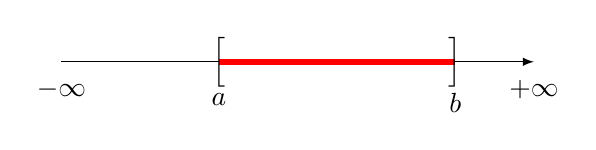
\begin{tikzpicture}[>=latex]
    \draw[->] (0,0) --(6,0);
    \draw[line width=2pt,color=red] (2,0)--(5,0);
    \node[] at (5,0) {\rouge{$\Big]$}};
    \node[] at (2,0) {\rouge{$\Big[$}};
    \node[below=8pt] at (5,0) {$b$};
    \node[below=3pt] at (0,0) {$-\infty$};
    \node[below=3pt] at (6,0) {$+\infty$};
    \node[below=8pt] at (2,0) {$a$};
\end{tikzpicture}\\
\hline
        $a < x \leq b$ & $x\in \intervalleof a b$ &
    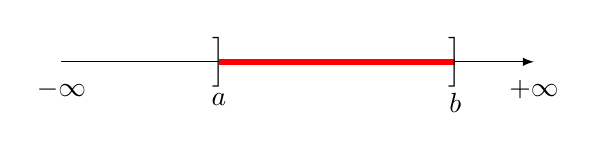
\begin{tikzpicture}[>=latex]
    \draw[->] (0,0) --(6,0);
    \draw[line width=2pt,color=red] (2,0)--(5,0);
    \node[] at (5,0) {\rouge{$\Big]$}};
    \node[] at (2,0) {$\Big]$};
    \node[below=8pt] at (5,0) {$b$};
    \node[below=3pt] at (0,0) {$-\infty$};
    \node[below=3pt] at (6,0) {$+\infty$};
    \node[below=8pt] at (2,0) {$a$};
\end{tikzpicture}\\
\hline
        $a \leq x < b$ & $x\in \intervallefo a b$ &
    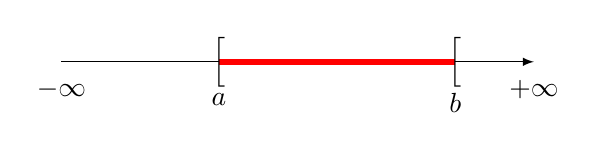
\begin{tikzpicture}[>=latex]
    \draw[->] (0,0) --(6,0);
    \draw[line width=2pt,color=red] (2,0)--(5,0);
    \node[] at (5,0) {$\Big[$};
    \node[] at (2,0) {\rouge{$\Big[$}};
    \node[below=8pt] at (5,0) {$b$};
    \node[below=3pt] at (0,0) {$-\infty$};
    \node[below=3pt] at (6,0) {$+\infty$};
    \node[below=8pt] at (2,0) {$a$};
\end{tikzpicture}\\
\hline
        $a < x < b$ & $x\in \intervalleoo a b$ &
    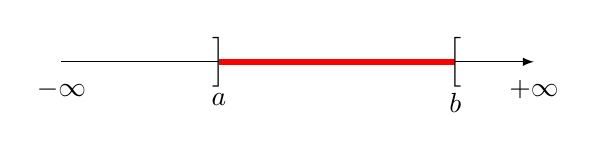
\begin{tikzpicture}[>=latex]
    \draw[->] (0,0) --(6,0);
    \draw[line width=2pt,color=red] (2,0)--(5,0);
    \node[] at (5,0) {$\Big[$};
    \node[] at (2,0) {$\Big]$};
    \node[below=8pt] at (5,0) {$b$};
    \node[below=3pt] at (0,0) {$-\infty$};
    \node[below=3pt] at (6,0) {$+\infty$};
    \node[below=8pt] at (2,0) {$a$};
\end{tikzpicture}\\
\hline
\end{tabular}
\end{center}

\subsubsection{Intervalles non bornés}
\begin{Defi}
    Un \iptb{intervalle non borné} est constitué de tous les nombres réels supérieurs ou inférieurs à un nombre réel.\par
    Par exemple, l'intervalle $\intervalleoo{a}{+\infty}$ est l'ensemble des nombres $x$ tels que $x > a$.
\end{Defi}

\begin{center}
\begin{tabular}{|>\bfseries c|>\bfseries c|>\bfseries m{7cm}|}
    \hline
        Inégalité & Notation & Représentation \\
    \hline
        $x \geq a $ & $x\in \intervallefo{a}{+\infty}$ &
    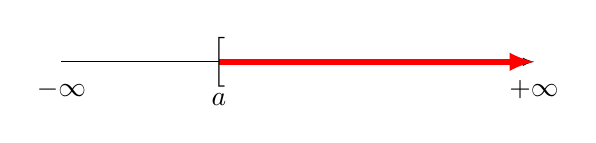
\begin{tikzpicture}[>=latex]
    \draw[->] (0,0) --(6,0);
    \draw[line width=2pt,color=red,->] (2,0)--(6,0);
    \node[] at (2,0) {\rouge{$\Big[$}};
    \node[below=3pt] at (0,0) {$-\infty$};
    \node[below=3pt] at (6,0) {$+\infty$};
    \node[below=8pt] at (2,0) {$a$};
\end{tikzpicture}\\
\hline
        $x > a $ & $x\in \intervalleoo{a}{+\infty}$ &
    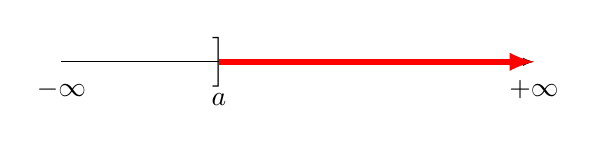
\begin{tikzpicture}[>=latex]
    \draw[->] (0,0) --(6,0);
    \draw[line width=2pt,color=red,->] (2,0)--(6,0);
    \node[] at (2,0) {{$\Big]$}};
    \node[below=3pt] at (0,0) {$-\infty$};
    \node[below=3pt] at (6,0) {$+\infty$};
    \node[below=8pt] at (2,0) {$a$};
\end{tikzpicture}\\
\hline
        $x \leq a $ & $x\in \intervalleof{-\infty}{a}$ &
    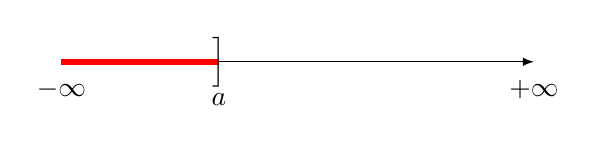
\begin{tikzpicture}[>=latex]
    \draw[->] (0,0) --(6,0);
    \draw[line width=2pt,color=red] (0,0)--(2,0);
    \node[] at (2,0) {\rouge{$\Big]$}};
    \node[below=3pt] at (0,0) {$-\infty$};
    \node[below=3pt] at (6,0) {$+\infty$};
    \node[below=8pt] at (2,0) {$a$};
\end{tikzpicture}\\
\hline
        $x < a $ & $x\in \intervalleoo{-\infty}{a}$ &
    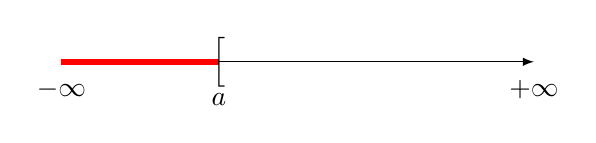
\begin{tikzpicture}[>=latex]
    \draw[->] (0,0) --(6,0);
    \draw[line width=2pt,color=red] (0,0)--(2,0);
    \node[] at (2,0) {{$\Big[$}};
    \node[below=3pt] at (0,0) {$-\infty$};
    \node[below=3pt] at (6,0) {$+\infty$};
    \node[below=8pt] at (2,0) {$a$};
\end{tikzpicture}\\
\hline
\end{tabular}
\end{center}

\subsubsection{Réunion et intersection}
\begin{Defi}
    \begin{enumerate}
        \item La \ipt{réunion} de deux intervalles $I$ et $J$, notée $I \cup J$, est l'ensemble des nombres réels appartenant à $I$ \textbf{ou} à $J$.
        \item L'\ipt{intersection} de deux intervalles $I$ et $J$, notée $I \cap J$, est l'ensemble des nombres réels appartenant à $I$ \textbf{et} à $J$.
    \end{enumerate}
\end{Defi}

\begin{Exemple}[s]
$\intervalleff{-2}{5} \cup \intervalleoo{0}{+\infty} = \intervallefo{-2}{\infty} \qq \intervalleff{-2}{5} \cap \intervalleoo{0}{+\infty} = \intervalleof 0 5$ \medskip

$\intervalleff{-2}{5} \cup \intervalleof{8}{15} = \intervalleff{-2}{5} \cup \intervalleof{8}{15}$ (on ne peut pas écrire la réunion sous forme d'un seul intervalle).\medskip

$\intervalleff{-2}{5} \cap \intervalleof{8}{15} = \emptyset$ (ensemble vide) : l'intersection ne contient aucun nombre.
\end{Exemple}\medskip

\begin{Rmq}
    On a les inclusions suivantes :
    \[I \subset I \cup J \qq J \subset I \cup J \qq I \cap J \subset I \qetq I \cap J \subset J.\]
\end{Rmq}

\subsection{Résolution d'inéquations}
\subsubsection{Inéquations du premier degré à une inconnue}

\begin{Prop}
    On peut ajouter un même nombre à chaque membre d'une inégalité pour obtenir ainsi une inégalité équivalente :
    \[a < b \qLRq a \rouge{\ +\ c } < b \rouge{\ +\ c}\]
\end{Prop}

\begin{Exemple}[s]
    $\begin{array}[t]{rcl}
        x + 4 & \leqslant & 5 \\
        x + 4 \rouge{\,-\,4} & \leqslant & 5 \rouge{\,-\,4} \\
        \multicolumn{3}{c}{\pfr{x\leqslant 1}}
    \end{array}$\quad
    $\begin{array}[t]{rcl}
        x - 3 & > & 0 \\
        x -3 \rouge{\,+\,3} & > & 0 \rouge{\,+\,3} \\
        \multicolumn{3}{c}{\pfr{x > 3}}
    \end{array}$
\end{Exemple}

\begin{Demo}
    $a$, $b$ et $c$ sont trois nombres tels que $a < b$. Donc :
    \[a - b < 0 \Leftrightarrow a - b + \underbrace{c - c}_{= 0} < 0 \Leftrightarrow a + c - (b + c) < 0 \Leftrightarrow \pfr{a + c < b + c}\]
\end{Demo}

\begin{Prop}
    On multiplie ou on divise les deux membres d'une inégalité par un même nombre $k$ non nul :
    \begin{itemize}
        \item si $k > 0$, alors : \quad $a < b \qLRq ka < kb$ ;
        \item si $k < 0$, alors : \quad $a < b \qLRq ka > kb$.
    \end{itemize}
\end{Prop}

\begin{Exemple}[s]
    $\begin{array}[t]{rcl}
        3x + 4 & < & 2 \\
        3x & < & -2 \\[7.5pt]
        \multicolumn{3}{c}{\pfr{x < \dfrac{-2}{3}}}
    \end{array}$\quad
    $\begin{array}[t]{rcl}
        \dfrac{x}{-2} + 6 & \geqslant & 0 \\[7.5pt]
        \dfrac{x}{-2} & \geqslant & -6 \\[7.5pt]
        \multicolumn{3}{c}{\pfr{x \rouge{\leqslant} 12}}
    \end{array}$
\end{Exemple}

\begin{Demo}
    On considère trois nombres $a$, $b$ et $k$ tels que $a > b$.\par
    $a - b$ est donc un nombre positif.\par
    On rappelle que le produit de deux nombres de même signe est positif, négatif sinon.
    \[\begin{array}{c@{\hspace*{3cm}}c}
        \underbar{\text{Si } k > 0} & \underbar{\text{Si } k < 0} \\[5pt]
        k(a - b) > 0 & k(a - b) < 0 \\
        \Leftrightarrow ka - kb > 0 & \Leftrightarrow ka - kb < 0 \\
        \Leftrightarrow \pfr{ka > kb} & \Leftrightarrow \pfr{ka < kb}
    \end{array}\]
\end{Demo}\medskip

\subsubsection{Résolution de problèmes}

\begin{Exemple}
    Dans un club de gym, deux formules sont proposées :
    \begin{description}
        \item[Formule A :] abonnement mensuel de \EUR{$18$} et \EUR{$5$} la séance.
        \item[Formule B :] abonnement mensuel de \EUR{$30$} et \EUR{$3$} la séance.
    \end{description}
    Déterminer par le calcul le nombre de séances minimum pour lequel la formule B est plus avantageuse.
\end{Exemple}\medskip

Voici les étapes de la résolution d'un problème en utilisant les inéquations :
\begin{enumerate}
    \item choix de l'inconnue ;
    \item trouver l'inéquation correspondant au problème ;
    \item résolution de l'inéquation ;
    \item réponse au problème.
\end{enumerate}\medskip

\end{document}

%------ Chapitre 02
    \documentclass[10pt,openright,twoside,french]{book}

\input philippe2013
\input philippe2013_cours
\input philippe2013_sections
\input philippe2013_chapitre


\begin{document}
\setcounter{chapter}{1}
\renewcommand\PartProgramme{Géométrie}
\chapter[Coordonnées d'un point dans le plan]{Coordonnées d'un point\\ dans le plan}\label{ch_coordonnees}

\section{Repère orthonormé}

\begin{Defi}
    Un \ipt{repère orthonormé} du plan $(O,I,J)$ est défini de façon unique par la donnée de trois points non alignés $O$, $I$ et $J$ tels que :
    \begin{itemize}
        \item $(OI) \bot (OJ)$ ;
        \item $OI = OJ$.
    \end{itemize}
    Le point $O$ est appelé \ipt{origine du repère}.\par
    La droite graduée $(OI)$, orientée de $O$ vers $I$, est appelé \ipt{axe des abscisses} et la droite graduée $(OJ)$, orientée de $O$ vers $J$, est appelée \ipt{axe des ordonnées}.\par
    La longueur $OI$ définit l'unité de longueur sur l'axe des abscisses et la longueur $OJ$ définit l'unité de longueur sur l'axe des ordonnées.\par
    Par définition, les deux axes sont perpendiculaires et les unités de longueur sont identiques.
\end{Defi}

\begin{center}
%  \begin{tikzpicture}[x={(0.5cm,0cm)},y={(0.4cm,0.5cm)}]]
%        %\draw[line width=1pt,color=gray!25,dashed] (-4,-4) grid (4,4);
%        \foreach \x in {-4,-3,...,4} \draw[color=gray!25,line width=1pt,dashed] (\x,-4)--(\x,4);
%        \foreach \x in {-4,-3,...,4} \draw[color=gray!25,line width=1pt,dashed] (-4,\x)--(4,\x);
%        \draw[->,blue](-4,0)--(4,0);
%        \draw[->,blue](0,-4)--(0,4);
%        \draw (0,0) node[below] {\footnotesize $O$};
%        \draw (1,-0.2) node[below] {\footnotesize $I$}; \draw (1,0) node {|};
%        \draw (0,1) node[left] {\footnotesize $J$}; \draw (0,1) node {--};
%        \draw (0,-4) node[below] {Repère du plan};
%    \end{tikzpicture}\qquad%
%    \begin{tikzpicture}[x={(0.5cm,0cm)},y={(0cm,0.25cm)}]]
%        %\draw[line width=1pt,color=gray!25,dashed] (-4,-4) grid (4,4);
%        \foreach \x in {-4,-3,...,4} \draw[color=gray!25,line width=1pt,dashed] (\x,-4)--(\x,4);
%        \foreach \x in {-4,-3,...,4} \draw[color=gray!25,line width=1pt,dashed] (-4,\x)--(4,\x);
%        \draw[->,blue](-4,0)--(4,0);
%        \draw[->,blue](0,-4)--(0,4);
%        \draw (0,0) node[below left] {\footnotesize $O$};
%        \draw (1,-0.2) node[below] {\footnotesize $I$}; \draw (1,0) node {|};
%        \draw (0,1) node[left] {\footnotesize $J$}; \draw (0,1) node {--};
%        \draw (0,-4) node[below] {Repère orthogonal};
%    \end{tikzpicture}\par\medskip
    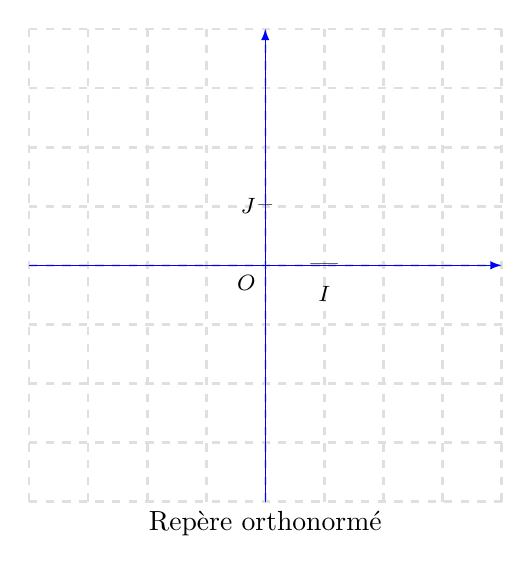
\begin{tikzpicture}[scale=0.75,>=latex]
        %\draw[line width=1pt,color=gray!25,dashed] (-4,-4) grid (4,4);
        \foreach \x in {-4,-3,...,4} \draw[color=gray!25,line width=1pt,dashed] (\x,-4)--(\x,4);
        \foreach \x in {-4,-3,...,4} \draw[color=gray!25,line width=1pt,dashed] (-4,\x)--(4,\x);
        \draw[->,blue](-4,0)--(4,0);
        \draw[->,blue](0,-4)--(0,4);
        \draw (0,0) node[below left] {\footnotesize $O$};
        \draw (1,-0.2) node[below] {\footnotesize $I$}; \draw (1,0) node {|};
        \draw (0,1) node[left] {\footnotesize $J$}; \draw (0,1) node {--};
        \draw (0,-4) node[below] {Repère orthonormé};
    \end{tikzpicture}
\end{center}

\section{Coordonnées d'un point}

On considère un point $M$ du plan dans un repère $(O,I,J)$ orthonormé.\par
On trace la parallèle à $(OJ)$ passant par $M$. Elle coupe l'axe des abscisses en $H$.\par
On trace la parallèle à $(OI)$ passant par $M$. Elle coupe l'axe des ordonnées en $K$.\medskip

\begin{Defi}
    \begin{enumerate}
        \item Sur l'axe $(OI)$, le nombre réel associé à $H$ est appelé \ipt{abscisse} du point $M$, que l'on note $x_M$.
        \item Sur l'axe $(OJ)$, le nombre réel associé à $K$ est appelé \ipt{ordonnée} du point $M$, que l'on note $y_M$.
        \item Le couple $(x_M \pv y_M)$ est alors appelé \ipt{coordonnées} du point $M$ et l'on note $M(x_M \pv y_M)$.
    \end{enumerate}
\end{Defi}\clearpage

\begin{Exemple}
\strut\par
\begin{minipage}{0.5\linewidth}
    Sur la figure ci-contre, l'abscisse de $M$ est égale à $3$ et son ordonnée est égale à $2,5$. On dira que les coordonnées de $M$ sont $(3 \pv 2,5)$ et on note $M(3 \pv 2,5)$.
\end{minipage}\quad
\begin{minipage}{0.4\linewidth}
\begin{center}
    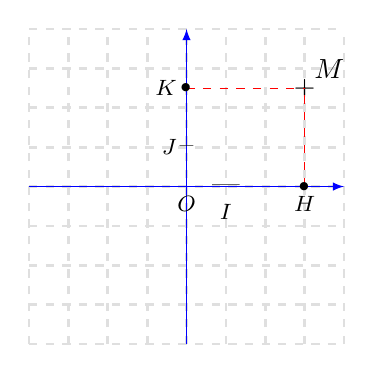
\begin{tikzpicture}[scale=0.5,>=latex]
        \foreach \x in {-4,-3,...,4} \draw[color=gray!25,line width=1pt,dashed] (\x,-4)--(\x,4);
        \foreach \x in {-4,-3,...,4} \draw[color=gray!25,line width=1pt,dashed] (-4,\x)--(4,\x);
        \draw[->,blue](-4,0)--(4,0);
        \draw[->,blue](0,-4)--(0,4);
        \draw (0,0) node[below] {\footnotesize $O$};
        \draw (1,-0.2) node[below] {\footnotesize $I$}; \draw (1,0) node {|};
        \draw (0,1) node[left] {\footnotesize $J$}; \draw (0,1) node {--};
        \draw (3,2.5) node[above right]{$M$}; \draw (3,2.5) node{$+$};
        \draw[dashed,red] (0,2.5)--(3,2.5); \draw (0,2.5) node[left]{\footnotesize$K$}; \draw (0,2.5) node{\rouge{$_\bullet$}};
        \draw[dashed,red] (3,0)--(3,2.5); \draw (3,0) node[below]{\footnotesize$H$}; \draw (3,0) node{\rouge{$_\bullet$}};
    \end{tikzpicture}
    \end{center}
\end{minipage}
\end{Exemple}

\begin{Rmq}
    Dans un  repère $(O,I,J)$, $A \in (OI) \Leftrightarrow y_A = 0$ et $B \in (OJ) \Leftrightarrow x_B = 0$.\par
    En particulier,  les coordonnées de l'origine du repère sont $(0 \pv 0)$, celle de $I$ sont $(1 \pv 0)$ et celle de $J$ sont $(0 \pv 1)$.\par
\end{Rmq}

\section{Distances dans un repère orthonormé}
On se place dans un repère \textbf{orthonormé} du plan $(O,I,J)$ et on considère deux points $A(x_A \pv y_A)$ et $B(x_B \pv y_B)$.\par\medskip

\begin{Prop}[(partiellement démontrée en exercice)]
    \begin{enumerate}
        \item Lorsque $x_A = x_B$, on pose $AB = y_B - y_A$ lorsque $y_B > y_A$ ou bien $AB = y_A - y_B$ lorsque $y_A > y_B$.
        \item Lorsque $y_A = y_B$, on pose $AB = x_B - x_A$ lorsque $x_B > x_A$ ou bien $AB = x_A - x_B$ lorsque $x_A > x_B$.
    \end{enumerate}
\end{Prop}\medskip

\begin{Rmq}
    Dans le premier cas, $(AB)$ est parallèle à l'axe des ordonnées et dans le second cas, $(AB)$ est parallèle à l'axe des abscisses.
\end{Rmq}\medskip

\begin{Exemple}
\strut

\begin{center}
\begin{tikzpicture}[>=latex]
        \draw[->,blue](-2.5,0)--(4,0);
        \draw[->,blue](0,-2)--(0,3.5);
        \draw (0,0) node[below left] {\footnotesize $O$};
        \draw (1,-0.1) node[below] {\footnotesize $I$}; \draw (1,0) node {|};
        \draw (0,1) node[left] {\footnotesize $J$}; \draw (0,1) node {--};
        \draw [dash pattern=on 5pt off 5pt] (-2,0)--(-2,2.5);
        \draw [dash pattern=on 5pt off 5pt] (1.5,0)-- (1.5,2.5);
        \draw [dash pattern=on 5pt off 5pt] (1,0.5)--(0,0.5);
        \draw [dash pattern=on 5pt off 5pt] (1,1.5)-- (0,1.5);
        \begin{scriptsize}
            \coordinate (A) at (-2,2.5); \draw (A) node[above left]{$A$}; \draw (-2,0) node[below] {$x_A$};
            \coordinate (B) at (1.5,2.5); \draw (B) node[above left]{$B$}; \draw (1.5,0) node[below] {$x_B$};
            \coordinate (C) at (1,1.5); \draw (C) node[right]{$C$}; \draw (0,1.5) node[left] {$y_C$};
            \coordinate (D) at (1,0.5); \draw (D) node[right]{$D$}; \draw (0,0.5) node[left]{$y_D$};
        \end{scriptsize}
        \draw (A) node {$\times$};\draw (B) node {$\times$};\draw (C) node {$\times$};\draw (D) node {$\times$};
        \draw[red] (A)--(B); \draw[red] (C)--(D);
        \draw (2.5,2) node[above right] {$AB = x_B - x_A$};
        \draw (2.5,2) node[below right] {$CD = y_C - y_D$};
\end{tikzpicture}
\end{center}
\end{Exemple}

\subsection{Calcul de distance}
\begin{Prop}
    La distance entre les points $A$ et $B$, autrement dit la longueur du segment $[AB]$, est égale à :
    \[AB = \sqrt{(x_B - x_A)^2 + (y_B - y_A)^2}\]
\end{Prop}\clearpage

\begin{Demo}
\begin{minipage}{0.55\linewidth}
On considère la figure ci-contre. Le point $C$ a pour coordonnées $(x_B \pv y_A)$ et, par conséquent, le triangle $ABC$ est rectangle en $C$.\par
D'après le théorème de Pythagore, on a \[AB^2 = AC^2 + BC^2.\]
Par construction, $A$ et $C$ ont la même ordonnée donc $AC^2 = (x_B - x_A)^2$. De même, puisque $B$ et $C$ ont la même abscisse, $BC^2 = (y_B - y_A)^2$.\par
Ainsi, $AB^2 = (x_B - x_A)^2 + (y_B - y_A)^2$ (qui est un nombre positif) donc finalement :
    \[AB = \sqrt{(x_B - x_A)^2 + (y_B - y_A)^2}\]
\end{minipage}\qquad
\begin{minipage}{0.4\linewidth}
\begin{center}
    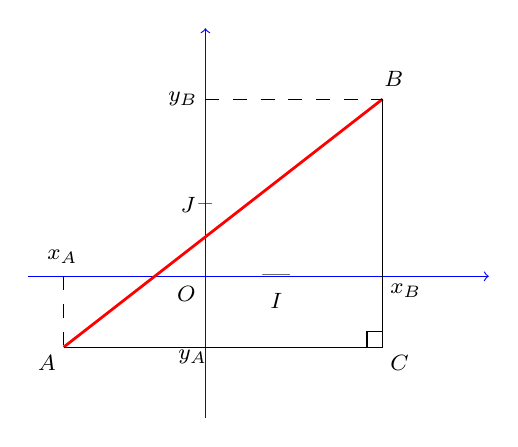
\begin{tikzpicture}[scale=0.9]
            \draw[->,blue](-2.5,0)--(4,0);
            \draw[->,blue](0,-2)--(0,3.5);
            \draw (0,0) node[below left] {\footnotesize $O$};
            \draw (1,-0.1) node[below] {\footnotesize $I$}; \draw (1,0) node {|};
            \draw (0,1) node[left] {\footnotesize $J$}; \draw (0,1) node {--};
            \draw (2.5,-0.78) -- (2.28,-0.78) -- (2.28,-1) -- (2.5,-1) -- cycle;
            \draw[line width=1pt,red] (-2,-1)-- (2.5,2.5);
            \draw (-2,-1)-- (2.5,-1);
            \draw (2.5,-1)-- (2.5,2.5);
            \draw [dash pattern=on 5pt off 5pt] (0,2.5)-- (2.5,2.5);
            \draw [dash pattern=on 5pt off 5pt] (-2,0)-- (-2,-1);
            \begin{scriptsize}
                \draw (-2,-1) node[below left] {\footnotesize$A$};
                \draw (2.66,2.78) node {\footnotesize$B$};
                \draw (2.5,-1) node[below right] {\footnotesize$C$};
                \draw (-0,2.5) node[left] {\footnotesize$y_B$};
                \draw (-2.02,0.28) node {\footnotesize$x_A$};
                \draw (-0.18,-1.14) node {\footnotesize$y_A$};
                \draw (2.5,0) node[below right] {\footnotesize$x_B$};
        \end{scriptsize}
    \end{tikzpicture}
\end{center}
\end{minipage}

\end{Demo}

\subsection{Milieu d'un segment}
\begin{Prop}
    On a appelle $P$ le milieu du segment $[AB]$. On a alors :
    \[x_P = \frac{x_A + x_B}{2} \qetq y_P = \frac{y_A + y_B}{2}.\]
\end{Prop}

\begin{Demo}
    \begin{minipage}{0.5\linewidth}
        \textbf{1\ier cas : $x_A = x_B$ ou $y_A = y_B$.}\par
        On suppose que $y_A = y_B$ et $x_B > x_A$. $P$ est le milieu de $[AB]$ si, et seulement si, $P \in [AB]$ et $PA = PB$.\par
        $P \in [AB] \Leftrightarrow y_P = y_A = y_B$ et on a bien $y_P = \frac{y_A + y_B}{2}$.\par
        $PA = PB \Leftrightarrow x_P - x_A = x_B - x_P \Leftrightarrow 2x_p = x_B + x_A$ et on a bien $x_P = \frac{x_A+ x_B}{2}$.
    \end{minipage}\quad
    \begin{minipage}{0.4\linewidth}
        \begin{center}
        \begin{tikzpicture}[scale=0.75]
                \begin{scriptsize}
                    \coordinate (A) at (0.5,2.5); \draw (A) node[above=5pt]{$A$};
                    \coordinate (C) at (0.5,0); \draw (C) node[below] {$x_A$};
                    \draw[dashed] (A)--(C);
                    \coordinate (B) at (5,2.5); \draw (B) node[above=5pt]{$B$};
                    \coordinate (D) at (5,0); \draw (D) node[below] {$x_B$};
                    \draw[dashed] (B)--(D);
                    \shorthandoff{!}
                    \coordinate (P) at ($ (A)!.5!(B) $); \draw (P) node {\rouge{$+$}} node[above=5pt] {$P$};
                    \coordinate(M) at ($(A)!.5!(P)$);\coordinate(N) at ($(A)!1.5!(P)$);
                    \shorthandon{!}
                    \coordinate (K) at (2.75,0); \draw (K) node {\rouge{$+$}} node[below=3pt] {$x_P$};
                \end{scriptsize}
                \draw (A) node {$+$};\draw (B) node {$+$};\draw (P) node {\rouge{$+$}};\draw (K) node {\rouge{$+$}};
                \draw[->,blue](-0.5,0)--(6,0);
                \draw[->,blue](0,-0.5)--(0,3.5);
                \draw (0,0) node[below left] {\footnotesize $O$};
                \draw[dashed] (0,2.5)--(B);
                \draw[dashed,red] (K)--(P);
                \draw (M) node{\violet{/\!\!/}};\draw (N) node{\violet{/\!\!/}};
        \end{tikzpicture}
        \end{center}
    \end{minipage}\bigskip

    \begin{minipage}{0.5\linewidth}
        \textbf{2\ieme cas : $x_A \neq x_B$ et $y_A \neq y_B$.}\par
        On note $C$ le point de coordonnées $(x_B \pv y_A)$ de façon à ce que le triangle $ABC$ soit rectangle en $C$. On appelle $K$ le milieu de $[AC]$ et $L$ celui de $[BC]$.\par
        On constate pour commencer que $(BC)$ est parallèle à l'axe des ordonnées car $x_B = x_C$ et que $(AC)$ est parallèle à l'axe des abscisses puisque $y_A = y_C$.
        Dans le triangle $ABC$, $P$ est le milieu de $[AB]$ et $K$ est celui de $[AC]$. D'après le théorème de la droite des milieux, on en déduit que $(PK)$ est parallèle à $(BC)$ et donc $(PK)$ est parallèle à $(OJ)$ donc $x_P = x_K = \frac{x_A + x_C}{2}$ donc $x_P = \frac{x_A + x_B}{2}$.\par
        En utilisant le point $L$, on obtiendrait de même $y_P = \frac{y_A + y_B}{2}$.
    \end{minipage}\quad
    \begin{minipage}{0.4\linewidth}
        \begin{center}
        \begin{tikzpicture}[scale=0.75]
                \begin{scriptsize}
                    \coordinate (A) at (0.5,1.5); \draw (A) node[above=5pt]{$A$};
                    \coordinate (C) at (0.5,0); \draw (C) node[below] {$x_A$};
                    \draw[dashed] (A)--(C);
                    \coordinate (B) at (5,3.5); \draw (B) node[above=5pt]{$B$};
                    \coordinate (D) at (5,0); \draw (D) node[below] {$x_B$};
                    \draw[dashed] (B)--(D);
                    \coordinate (Z) at (5,1.5);
                    \shorthandoff{!}
                    \coordinate (P) at ($ (A)!.5!(B) $); \draw (P) node {\rouge{$+$}} node[above=5pt] {$P$};
                    \coordinate(M) at ($(A)!.5!(P)$);\coordinate(N) at ($(A)!1.5!(P)$);
                    \coordinate(W) at ($(A)!.5!(Z)$);\coordinate(U) at ($(B)!.5!(Z)$);
                    \shorthandon{!}
                    \coordinate (K) at (2.75,0); \draw (K) node {\rouge{$+$}} node[below=5pt] {$x_P$};
                    \draw (Z) node[right]{$C$};
                    \draw (W) node[below right] {$K$};
                    \draw (U) node[right]{$L$};
                \end{scriptsize}
                \draw (A) node {$+$};\draw (B) node {$+$};\draw (P) node {\rouge{$+$}};\draw (K) node {\rouge{$+$}};
                \draw[->,blue](-0.5,0)--(6,0);
                \draw[->,blue](0,-0.5)--(0,3.5);
                \draw (0,0) node[below left] {\footnotesize $O$};
                \draw (A)--(B)--(Z)--cycle;
                \draw (M) node{\violet{$||$}};\draw (N) node{\violet{$||$}};
                \draw[red] (P)--(W); \draw[dashed,red] (K)--(W);
                \draw (U) node{$+$};
        \end{tikzpicture}
        \end{center}
    \end{minipage}
\end{Demo}

\section{Applications}
\begin{Exemple}[s]
On se place dans un repère orthonormé $(O,I,J)$ :
\begin{enumerate}
    \item Que peut-on dire du triangle $ABC$ tel que $A(-4 \pv 3)$, $B(-4\pv-5)$ et $C(3\pv-1)$ ?
    \item On considère le point $D$ de coordonnées $(x_D \pv y_D)$. On appelle $E$, son symétrique par rapport à $(OI)$ et $F$ son symétrique par rapport à $(OJ)$. Calculer les coordonnées de $E$ et $F$ en fonction de celles de $D$.
    \item On considère le point $G$ de coordonnées $(x_G \pv y_G)$ et on construit $H$, son symétrique par rapport à $O$. Calculer les coordonnées de $H$ en fonction de celles de $G$.
    \item On considère les quatre points suivants :
    \[K(-4\pv -1) \qq I(1 \pv 0) \qq L(2\pv2) \qetq M(-3\pv1).\]
    Démontrer de deux façons différentes que le quadrilatère $KILM$ est un parallélogramme.
\end{enumerate}
\end{Exemple}

\end{document}


%------ Chapitre 03
    \documentclass[10pt,openright,twoside,french]{book}

\input philippe2013
\input philippe2013_cours
\input philippe2013_sections
\input philippe2013_chapitre


\begin{document}
\setcounter{chapter}{2}
\renewcommand\PartProgramme{Fonctions}
\chapter[Généralités sur les fonctions]{Généralités sur\\ les fonctions}\label{ch_gen_fonctions}

\section{Notions}

\begin{Defi}
    Soit $\calig D_f$ un ensemble de nombres réels (généralement un intervalle ou une réunion d'intervalles).
    Définir une \ipt{fonction} $f$ sur $\calig D_f$, c'est associer à tout nombre $x$ de $\calig D_f$ un réel unique, noté $f(x)$ et appelé \ipt{image} de $x$ par $f$.\par
    $x$ est appelée la \ipt{variable} et $f(x)$ est la valeur prise par la fonction $f$ pour la valeur $x$.\par
    L'ensemble $\calig D_f$ est appelé \ipt{ensemble de définition} de $f$ (ou domaine de définition).
\end{Defi}\medskip

\textbf{Notation :}\quad La phrase : \textit{\og~La fonction $f$ qui, au nombre $x$, associe le nombre $f(x)$~\fg}\par
\textcolor{white}{\textbf{Notation }\quad} peut se noter de la façon suivante : $f : x \mapsto f(x)$.\medskip

\begin{Exemple}[s]
    \begin{enumerate}
        \item Soit $g$ la fonction qui, à $x$, associe le nombre $2x^2 - 1$.\par Elle est définie par $g(x) = 2x^2 -1$ et on note : $g : x \mapsto 2x^2 - 1.$
        \item Si on considère la taille associée à un individu, on définit une fonction : \textit{individu} $\mapsto$ \textit{taille}.
        \item	Si on considère le prix de vente d'un litre d'essence dans une ville, on ne définit pas une fonction car pour un même type d'essence, il peut exister plusieurs prix en fonction des stations service.
    \end{enumerate}
\end{Exemple}\medskip

Pour avoir une idée visuelle de la fonction, il est souvent utile de la représenter graphiquement dans un repère orthonormé. On a alors la définition suivante :\medskip

\begin{Defi}
Soit $f$ une fonction définie sur $\calig D_f$.\par
Dans un repère du plan, la \ipt{courbe représentative} $\calig C_f$ de $f$ est l'ensemble des points $M$ de coordonnées $(x_M \pv y_M)$ telles que :
\begin{itemize}
    \item $x_M$ décrit l'ensemble de définition $\calig D_f$ ;
    \item $y_M$ est l'image de $x_M$ par $f$ : $y_M = f(x_M)$.
\end{itemize}
\end{Defi}\medskip

\begin{Rmq}
    On dit que $\calig C_f$ a pour équation $y = f(x)$ dans le repère choisi.
\end{Rmq}\medskip

\begin{center}
    \begin{tikzpicture}[scale=1.2]
        \draw[->,blue] (-1.75,0)--(4,0);
        \draw[->,blue] (0,-0.25)--(0,3);
        \draw[color=red,line width=1pt] plot[domain=-1.25:3.6,samples=200] (\x,{cos(deg(\x))+1.5});
        \coordinate (M) at (1.5,{cos(deg(1.5))+1.5}); \draw (M) node{\large $+$};
        \draw[dashed] (1.5,0)|-(0,{cos(deg(1.5))+1.5});
        \begin{scriptsize}
            \draw (M) node[above right]{$M$};
            \draw (1.5,0) node[below] {$x_M$};
            \draw (0,{cos(deg(1.5))+1.5}) node[left] {$y_M=f(x_M)$};
            \draw (3.5,{cos(deg(3.5))+1.5}) node[above] {$\calig C_f$};
        \end{scriptsize}
    \end{tikzpicture}
\end{center}\clearpage

\begin{Defi}
    On considère une fonction $f : x \mapsto f(x)$.\par
    Soit $y$ un nombre réel pour lequel il existe $x \in \calig D_f$ tel que $y = f(x)$.\par
    On dit alors que $x$ est un \ipt{antécédent} de $y$ par $f$.
\end{Defi}

\begin{Rmq}
    D'après les définitions précédentes, on en déduit que l'image d'un nombre de $\calig D_f$ existe toujours et est \textbf{unique} alors qu'un nombre peut avoir plusieurs antécédents (voire aucun).
\end{Rmq}

\section{Définir une fonction}
\subsection{À partir d'une courbe représentative}

\begin{tabularx}{\linewidth}{|X|X|X|}
\hline
\textbf{Ensemble de définition} & \textbf{Lecture d'image} & \textbf{Lecture d'antécédents} \\
\hline
%-- colonne 1
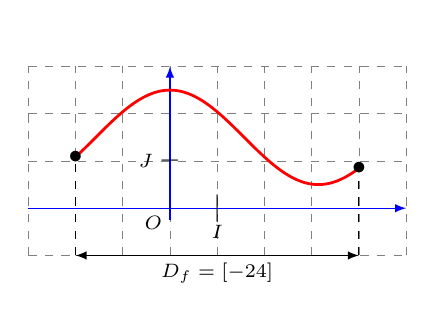
\begin{tikzpicture}[scale=0.6,>=latex]
    \draw[dashed,very thin,color = gray] (-3,-1) grid (5,3);
    \draw[->,blue] (-3,0)--(5,0);
    \draw[->,blue] (0,-0.25)--(0,3);
    \draw[color=red,line width=1pt] plot[domain=-2:4,samples=200] (\x,{cos(deg(\x))+1.5});
    \draw[dashed] (-2,-1)--(-2,{cos(deg(-2))+1.5});
    \draw[dashed] (4,-1)--(4,{cos(deg(4))+1.5});
    \draw (-2,{cos(deg(-2))+1.5}) node{\rouge{$ \bullet$}};
    \draw (4,{cos(deg(4))+1.5}) node{\rouge{$ \bullet$}};
    \draw (1,0) node {$|$};\draw (0,1) node {$-$};
    \draw (0,3.5) node {\textcolor{white}{a}};
    \begin{scriptsize}
        \draw[<->] (-2,-1)--(4,-1) node[midway,below] {$\calig D_f = [-2 \pv 4]$};
        \draw (0,0) node[below left]{$O$};
        \draw (1,-0.2) node[below]{$I$};
        \draw (-0.2,1) node[left]{$J$};
    \end{scriptsize}
\end{tikzpicture}&
%-- colonne 2
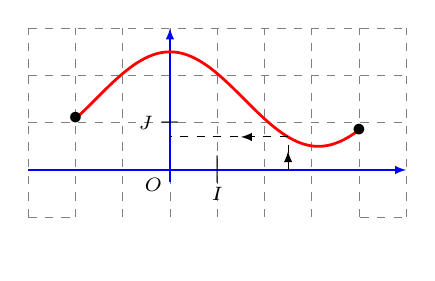
\begin{tikzpicture}[scale=0.6,>=latex]
    \draw[dashed,very thin,color = gray] (-3,-1) grid (5,3);
    \draw[->,blue] (-3,0)--(5,0);
    \draw[->,blue] (0,-0.25)--(0,3);
    \draw[color=red,line width=1pt] plot[domain=-2:4,samples=200] (\x,{cos(deg(\x))+1.5});
    \draw (-2,{cos(deg(-2))+1.5}) node{\rouge{$ \bullet$}};
    \draw (4,{cos(deg(4))+1.5}) node{\rouge{$ \bullet$}};
    \draw (1,0) node {$|$};\draw (0,1) node {$-$};
    \draw[dashed] (2.5,0)|-(0,{cos(deg(2.5))+1.5});
    \draw[->](2.5,0.3)--(2.5,0.4);
    \draw[->](1.6,{cos(deg(2.5))+1.5})--(1.5,{cos(deg(2.5))+1.5});
    \begin{scriptsize}
        \draw (0,0) node[below left]{$O$};
        \draw (1,-0.2) node[below]{$I$};
        \draw (-0.2,1) node[left]{$J$};
        \draw[white] (-2,-1)--(4,-1) node[midway,below] {\textcolor{white}{$\calig D_f = [-2 \pv 4]$}};
    \end{scriptsize}
\end{tikzpicture}&
%-- colonne 3
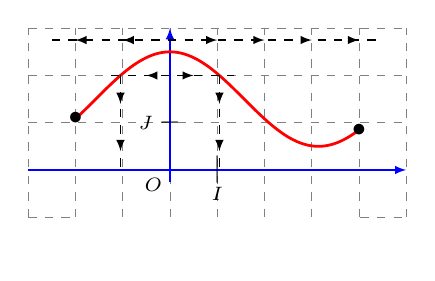
\begin{tikzpicture}[scale=0.6,>=latex]
    \draw[dashed,very thin,color = gray] (-3,-1) grid (5,3);
    \draw[->,blue] (-3,0)--(5,0);
    \draw[->,blue] (0,-0.25)--(0,3);
    \draw[color=red,line width=1pt] plot[domain=-2:4,samples=200] (\x,{cos(deg(\x))+1.5});
    \draw (-2,{cos(deg(-2))+1.5}) node{\rouge{$ \bullet$}};
    \draw (4,{cos(deg(4))+1.5}) node{\rouge{$ \bullet$}};
    \draw (1,0) node {$|$};\draw (0,1) node {$-$};
    \draw[dashed] (-2.5,2.75)--(4.5,2.75);
    \draw[dashed] ({acos((0.5))*pi/180},2)--({acos((0.5))*pi/180},0);
    \draw[dashed] ({-acos((0.5))*pi/180},2)--({-acos((0.5))*pi/180},0);
    \draw[dashed] ({-acos((0.5))*pi/180-0.2},2)--({acos((0.5))*pi/180+0.3},2);
    \draw[->](-0.4,2)--(-0.5,2);
    \draw[->](0.4,2)--(0.5,2);
    %
    \draw[->] ({acos((0.5))*pi/180},1.5)--({acos((0.5))*pi/180},1.4);
    \draw[->] ({-acos((0.5))*pi/180},1.5)--({-acos((0.5))*pi/180},1.4);
    \draw[->] ({acos((0.5))*pi/180},0.5)--({acos((0.5))*pi/180},0.4);
    \draw[->] ({-acos((0.5))*pi/180},0.5)--({-acos((0.5))*pi/180},0.4);
    %
    \draw[->] (-0.9,2.75)--(-1,2.75);
    \draw[->] (0.9,2.75)--(1,2.75);
    \draw[->] (-1.9,2.75)--(-2,2.75);
    \draw[->] (1.9,2.75)--(2,2.75);
    \draw[->] (2.9,2.75)--(3,2.75);
    \draw[->] (3.9,2.75)--(4,2.75);
    \begin{scriptsize}
        \draw (0,0) node[below left]{$O$};
        \draw (1,-0.2) node[below]{$I$};
        \draw (-0.2,1) node[left]{$J$};
        \draw[white] (-2,-1)--(4,-1) node[midway,below] {\textcolor{white}{$\calig D_f = [-2 \pv 4]$}};
    \end{scriptsize}
\end{tikzpicture} \\
\hline
Lecture de l'ensemble de définition sur l'axe des abscisses. &
Image d'un nombre sur l'axe des ordonnées. Ici, l'image de $2,5$ est environ $0,8$. &
Lecture d'antécédents sur l'axe des abscisses. Ici, $2$ a pour antécédent environ $-1$ et $1$. $2,75$ n'a pas d'antécédent.\\
\hline
\end{tabularx}\bigskip

\subsection{À partir d'un tableau}
On considère la fonction $f$ définie de la façon suivante :

\begin{center}
\begin{tabular}{|*{6}{c|}}
\hline
$x$ & $-2$ & $-1$ & $0$ & $1$ & $2$ \\
\hline
$f(x)$ & $1$ & $3$ & $8$ & $10$ & $3$ \\
\hline
\end{tabular}
\end{center}\bigskip

\begin{description}
    \item[Ensemble de définition.] La fonction n'est définie que pour les valeurs de $x$ écrites sur la première ligne du tableau. En dehors de ces nombres, on ne sait pas ce qu'il se passe.
    \item[Lecture d'image.] On sait que l'image de $x$ est $f(x)$ : on lit l'image d'un nombre de la première ligne dans la deuxième ligne. Par exemple, $f(1) = 10$.
    \item[Lecture d'antécédents.] Les antécédents se lisent sur la première ligne. Le nombre $3$ en a deux : $-1 $ et $2$. Le nombre $-2$ n'a pas d'antécédent.
\end{description}\bigskip

\subsection{À partir d'une formule}
\begin{Rmq}
    Connaître une fonction $f$ à partir d'une formule explicite permet d'avoir de nombreux renseignements. En particulier :
    \begin{itemize}
        \item on peut calculer l'image de n'importe quel nombre de l'ensemble de définition ;
        \item une formule permet de traduire le lien existant entre deux quantités.
        \item trouver un antécédent $a$ d'un nombre connu $b$ revient à résoudre l'équation $f(a) = b$.
    \end{itemize}
\end{Rmq}\clearpage

\begin{Exemple}
    Le poids idéal en fonction de la taille en $cm$ d'un homme et d'une femme adulte est calculé respectivement à l'aide des fonctions $h$ et $f$ ci-dessous :
    \[h(t) = t - 100 - \dfrac{t - 150}{4} \qquad f(t) =  t - 100 - \dfrac{t - 150}{2,5}\]
    \begin{enumerate}
        \item Quelles sont les deux quantités liées par chaque formule ? Quelle est celle qui dépend de l'autre ?
        \item Calculer le poids idéal d'un homme mesurant $1,75~m$.
        \item Calculer le poids idéal d'une femme mesurant $1,70~m$.
        \item Le nombre $59$ est-il l'image ou l'antécédent de $165$ par la fonction $f$ ?
        \item Calculer l'antécédent de $50$ par la fonction $f$ et interpréter le résultat.
    \end{enumerate}
\end{Exemple}



\end{document}

%------ Chapitre 04
    \documentclass[10pt,openright,twoside,french]{book}

\input philippe2013
\input philippe2013_cours
\input philippe2013_sections
\input philippe2013_chapitre

\setcounter{chapter}{3}
\begin{document}

\renewcommand\PartProgramme{Géométrie}
\chapter[\'Equations de droites]{\'Equations de \\ droites}\label{ch_equations_droites}

On se place dans un repère orthonormé \OIJ.\par Une droite peut alors être parallèle à l'axe des ordonnées (cas n°1) ou bien sécante à l'axe des ordonnées (cas n°2).

\section{Caractérisation analytique d'une droite}\index{equation@équation!équation de droite}

\begin{minipage}{0.6\textwidth}
\textbf{Cas n°1 :} Une droite est parallèle à l'axe des ordonnées si et seulement si tous les points situés sur cette droite ont la même abscisse.

\begin{Prop}\index{equation@équation!équation réduite}
    Toute droite $(d)$ parallèle à l'axe des ordonnées a une équation \iptb{réduite} de la forme $x = k$ ($k \in \R$).
\end{Prop}
\end{minipage}%
\begin{minipage}{0.4\textwidth}
    \begin{center}
        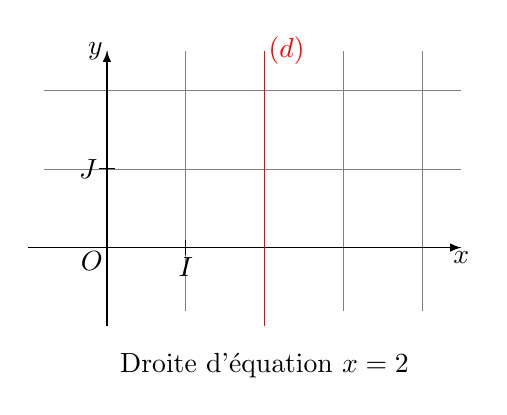
\begin{tikzpicture}[>=latex]
            \draw[help lines] (-0.8,-0.8) grid (4.5,2.5);
            \draw[->] (-1,0) -- (4.5,0) node[below=-2pt] {$x$};
            \draw[->] (0,-1) -- (0,2.5) node[left=-2pt] {$y$};
            \coordinate (O) at (0,0); \draw (O) node[below left = -2pt] {$O$};
            \coordinate (I) at (1,0); \draw (I) node[below] {$I$}; \draw (1,-0.1)--(1,0.1);
            \coordinate (J) at (0,1); \draw (J) node[left] {$J$}; \draw (-0.1,1)--(0.1,1);
            \draw[red] (2,-1) -- (2,2.5) node[right=-2pt] {$(d)$};
            \draw (2,-1.5) node {Droite d'équation $x = 2$};
        \end{tikzpicture}
    \end{center}
\end{minipage}

\begin{minipage}{0.6\textwidth}
\textbf{Cas n°2 :} Une droite qui coupe l'axe des ordonnées est la représentation d'une fonction affine. Réciproquement, une fonction affine a pour représentation graphique une droite sécante à l'axe des ordonnées.

\begin{Prop}\index{equation@équation!équation réduite}
    Toute droite $(d)$ sécante à l'axe des ordonnées a une équation \iptb{réduite} de la forme $y = mx + p$ ($m \in \R$ et $p \in \R$).
\end{Prop}
\end{minipage}%
\begin{minipage}{0.4\textwidth}
    \begin{center}
        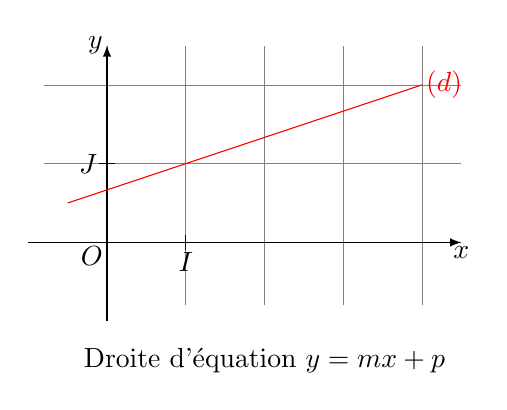
\begin{tikzpicture}[>=latex]
            \draw[help lines] (-0.8,-0.8) grid (4.5,2.5);
            \draw[->] (-1,0) -- (4.5,0) node[below=-2pt] {$x$};
            \draw[->] (0,-1) -- (0,2.5) node[left=-2pt] {$y$};
            \coordinate (O) at (0,0); \draw (O) node[below left = -2pt] {$O$};
            \coordinate (I) at (1,0); \draw (I) node[below] {$I$}; \draw (1,-0.1)--(1,0.1);
            \coordinate (J) at (0,1); \draw (J) node[left] {$J$}; \draw (-0.1,1)--(0.1,1);
            \draw[red] (-0.5,0.5) -- (4,2) node[right=-2pt] {$(d)$};
            \draw (2,-1.5) node {Droite d'équation $y = mx + p$};
        \end{tikzpicture}
    \end{center}
\end{minipage}

\begin{minipage}{0.6\textwidth}
\textbf{Cas particulier :} Lorsque $m = 0$, on trouve une équation de la forme $y = p$ ($p \in \R$). Dans ce cas, la droite $(d)$ est parallèle à l'axe des abscisses. Tous les points de cette droite ont la même ordonnée. Mais elle est toujours sécante à l'axe des ordonnées : c'est un cas particulier du cas n°2.
\end{minipage}%
\begin{minipage}{0.4\textwidth}
    \begin{center}
        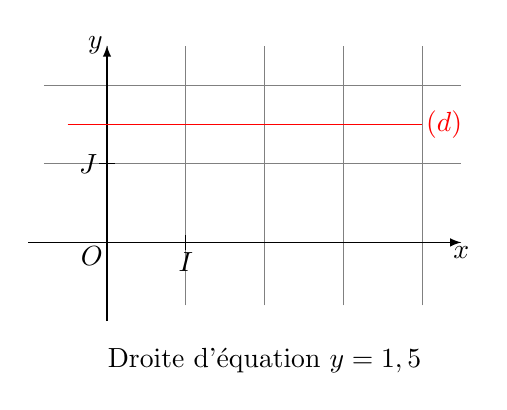
\begin{tikzpicture}[>=latex]
            \draw[help lines] (-0.8,-0.8) grid (4.5,2.5);
            \draw[->] (-1,0) -- (4.5,0) node[below=-2pt] {$x$};
            \draw[->] (0,-1) -- (0,2.5) node[left=-2pt] {$y$};
            \coordinate (O) at (0,0); \draw (O) node[below left = -2pt] {$O$};
            \coordinate (I) at (1,0); \draw (I) node[below] {$I$}; \draw (1,-0.1)--(1,0.1);
            \coordinate (J) at (0,1); \draw (J) node[left] {$J$}; \draw (-0.1,1)--(0.1,1);
            \draw[red] (-0.5,1.5) -- (4,1.5) node[right=-2pt] {$(d)$};
            \draw (2,-1.5) node {Droite d'équation $y = 1,5$};
        \end{tikzpicture}
    \end{center}
\end{minipage}

\begin{Defi}
    Considérons une droite $(d)$ dont l'équation réduite est de la forme : $y = mx + p$.\par
    Le nombre $m$ est appelé \ipt{c{\oe}fficient directeur} de la droite $(d)$. Ce \coef nous donne une indication sur l'inclinaison de la droite.\par
    Le nombre $p$ est appelé \ipt{ordonnée à l'origine}. En effet, lorsque $x = 0$ (origine de l'axe des abscisse), l'ordonnée $y$ est égale à $p$.
\end{Defi}

\section{Tracer une droite dans un repère}
Une droite d'équation $x = k$ passe par le point de coordonnées $(k \pv 0)$ et est parallèle à l'axe des ordonnées.\par
Une droite d'équation $y = p$ passe par le point de coordonnées $(0 \pv p)$ et est parallèle à l'axe des abscisses.\par
Pour représenter une droite d'équation $y = mx + p$, il faut et il suffit de connaître deux points appartenant à cette droite.

\begin{Exemple}[s]
    \begin{enumerate}
        \item Tracer la droite $(\Delta)$ d'équation $y = -2x + 3$.\par
        Puisqu'il faut deux points, choisissons arbitrairement deux valeurs de $x$ et calculons les valeurs de $y$ correspondantes.\par
        $x = 0$ : $y = -2 \times 0 + 3 = 3$ donc $A(0 \pv 3) \in (\Delta)$.\par
        $x = 1$ : $y = -2 \times 1 + 3 = 1$ donc $B(1 \pv 1) \in (\Delta)$.

        \item  Tracer la droite $(\Delta')$ d'équation $y = \frac 13 x - 1$.\par
        Puisqu'il faut deux points, choisissons arbitrairement deux valeurs de $x$ et calculons les valeurs de $y$ correspondantes.\par
        $x = 0$ : $y = \frac 13 \times 0 -1 = -1$ donc $C(0 \pv -1) \in (\Delta')$.\par
        $x = 3$ : $y = \frac13 \times 3 - 1 = 0$ donc $D(3 \pv 0) \in (\Delta)$.
    \end{enumerate}
        \begin{center}
            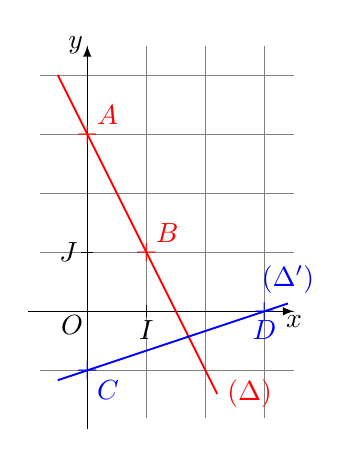
\begin{tikzpicture}[>=latex,scale=0.75]
                \draw[help lines] (-0.8,-1.8) grid (3.5,4.5);
                \draw[->] (-1,0) -- (3.5,0) node[below=-2pt] {$x$};
                \draw[->] (0,-2) -- (0,4.5) node[left=-2pt] {$y$};
                \coordinate (O) at (0,0); \draw (O) node[below left = -2pt] {$O$};
                \coordinate (I) at (1,0); \draw (I) node[below] {$I$}; \draw (1,-0.1)--(1,0.1);
                \coordinate (J) at (0,1); \draw (J) node[left] {$J$}; \draw (-0.1,1)--(0.1,1);
                \draw[color=red,line width=0.7pt] plot[domain=-0.5:2.2,samples=200] (\x,{-2*\x+3}) node[right] {$(\Delta)$};
                \draw[red] (0,3) node {$+$} node[above right] {$A$};
                \draw[red] (1,1) node {$+$} node[above right] {$B$};
                \draw[color=blue,line width=0.7pt] plot[domain=-0.5:3.4,samples=200] (\x,{\x/3-1}) node[above] {$(\Delta')$};
                \draw[blue] (0,-1) node {$+$} node[below right] {$C$};
                \draw[blue] (3,0) node {$+$} node[below] {$D$};
            \end{tikzpicture}
        \end{center}
\end{Exemple}

\section{Déterminer l'équation d'une droite}
\subsection{Cas n°1}
Une droite parallèle à l'axe des ordonnées a pour équation $x = k$.\par
Si on connaît la représentation graphique de la droite, il suffit ensuite de lire graphiquement la valeur de $k$. Sinon, en connaissant deux points, il suffit de lire leur abscisse commune.\medskip

\begin{Exemple}
    Déterminer l'équation de la droite passant par les points $K(-2 \pv 3)$ et $L(-2 \pv 6)$.\par
    Ces deux points ont la même abscisse donc la droite $(KL)$ est parallèle à l'axe des ordonnées et a pour équation $x = -2$.
\end{Exemple}

\subsection{Cas n°2}
Une droite sécante à l'axe des ordonnées à une équation de la forme $y = mx + p$. Deux points situés sur cette droite n'ont pas la même abscisse.\par

Lorsque l'on connaît les coordonnées de deux points de la droite, on détermine d'abord le \coef directeur puis on résoud une équation pour déterminer l'ordonnée à l'origine.

\begin{Prop}
    Soient $K(x_K \pv y_K)$ et $L(x_L \pv y_L)$ deux points dans un repère tel que $x_K \neq x_L$.\par
    Le \coef directeur de la droite $(KL)$ est : \[m = \frac{y_K - y_L}{x_K - x_L}.\]
\end{Prop}\clearpage

\begin{Demo}
    $K \in (KL)$ donc $y_K = mx_K + p$. De même, puisque $L \in (KL)$ alors $y_L = mx_L + p$.\par
    Ainsi,
    $\begin{array}[t]{rcl}
        y_K - y_L & = & mx_K + p - (mx_L + p)\\ &=& mx_K + p - mx_L - p\\ &=& mx_K - mx_L\\ &=& m(x_K - x_L)\end{array}$\medskip

        Puisque $x_K \neq x_L$, alors $x_K - x_L \neq 0$ et en divisant par $x_K - x_L$, on obtient :
        \[m = \frac{y_K - y_L}{x_K - x_L}.\]
\end{Demo}

\begin{Rmq}
    Lorsque l'on passe d'un point d'une droite à une autre en augmentant l'abscisse de $1$, alors la variation des ordonnées est donnée par $m$.
\end{Rmq}

\begin{Exemple}
    Déterminer l'équation de la droite $(d)$ passant par les points $A(3 \pv 4)$ et $(5 \pv -2)$.\par\medskip
    Les deux points n'ont pas la même abscisse donc l'équation réduite de la droite $(d)$ est de la forme $y = mx + p$.\par
    \begin{multicols}{2}
    \begin{description}
        \item[Calcul de $m$ :] $\begin{array}[t]{rcl}
                                                    m & = & \frac{y_A - y_B}{x_A - x_B}\\[10pt]
                                                        & = & \frac{4 - (-2)}{3 - 5}\\[10pt]
                                                        & = & \frac{6}{-2}\\[10pt]
                                                    m &= & -3
                                                \end{array}$
        \item[Calcul de $p$ :] Puisque $A \in (d)$ alors les coordonnées de $A$ vérifient l'équation de $(d)$ :
        \[\begin{array}{ll}
            & y_A = mx_A + p \\
            \Leftrightarrow & 4 = -3 \times 3 + p \\
            \Leftrightarrow & 4 = -9 + p \\
            \Leftrightarrow & p = 4 + 9 \\
            \Leftrightarrow & p = 13
        \end{array}\]
    \end{description}
        \end{multicols}
        La droite $(d)$ a donc pour équation : $y = -3x + 13$.
\end{Exemple}

\begin{Exemple}
    Déterminer l'équation de la droite $(d')$ dont voici la représentation graphique.

        \begin{center}
            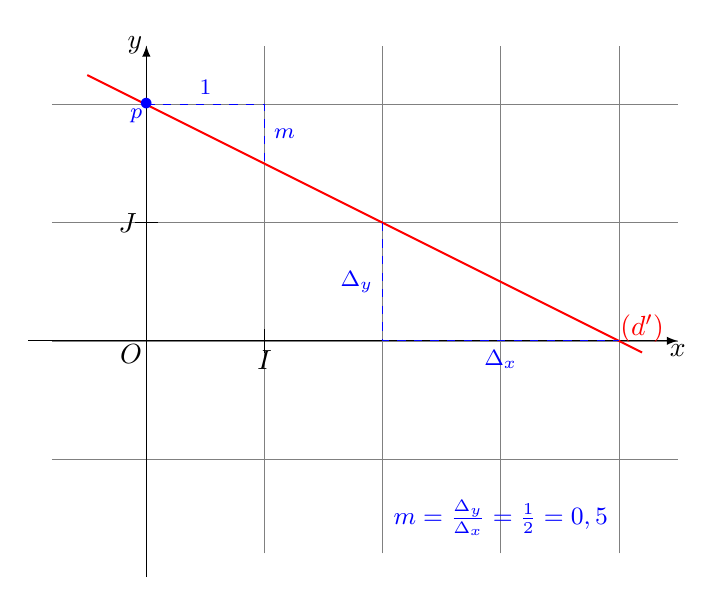
\begin{tikzpicture}[>=latex,scale=1.5]
                \draw[help lines] (-0.8,-1.8) grid (4.5,2.5);
                \draw[->] (-1,0) -- (4.5,0) node[below=-2pt] {$x$};
                \draw[->] (0,-2) -- (0,2.5) node[left=-2pt] {$y$};
                \coordinate (O) at (0,0); \draw (O) node[below left = -2pt] {$O$};
                \coordinate (I) at (1,0); \draw (I) node[below] {$I$}; \draw (1,-0.1)--(1,0.1);
                \coordinate (J) at (0,1); \draw (J) node[left] {$J$}; \draw (-0.1,1)--(0.1,1);
                \draw[color=red,line width=0.7pt] plot[domain=-0.5:4.2,samples=200] (\x,{-0.5*\x+2}) node[above] {$(d')$};
                \draw[blue, dashed] (0,2) -- (1,2) node[above,midway] {\footnotesize $1$} -- (1,1.5) node[right,midway] {\footnotesize $m$};
                \draw[blue, dashed] (2,1) -- (2,0) node[left,midway] {\footnotesize $\Delta_y$} -- (4,0) node[below,midway] {\footnotesize $\Delta_x$};
                \draw[blue] (0,2) node{$\bullet$} node[below left = -2pt] {\footnotesize $p$};
                \draw[blue] (3,-1.5) node {\small $m = \frac{\Delta_y}{\Delta_x} = \frac 12 = 0,5$};
            \end{tikzpicture}
        \end{center}
        La droite $(d')$ a pour équation : $y = \frac 1 2 x + 2$.
\end{Exemple}\clearpage

\section{Applications}
\subsection{Droites parallèles}
\begin{Rmq}[s]
    \begin{enumerate}
        \item Les droites qui ont une équation de la forme $x = k$ sont toutes parallèles à l'axe des ordonnées et elles sont donc parallèles entre elle.
        \item Une droite d'équation $x = k$ et une droite d'équation $y = mx + p$ sont sécantes car la première est parallèle à l'axe des ordonnées et pas la suivante.
    \end{enumerate}
\end{Rmq}

\begin{Prop}
    Une droite $(d)$ d'équation $y = mx + p$ et une droite $(d')$ d'équation $y = m'x + p'$ sont parallèles si, et seulement si, elles ont le même \coef directeur :
    \[(d) /\!/ (d') \quad \Leftrightarrow \quad m = m'\]
\end{Prop}

\begin{Demo}
On se place dans la situation suivante : les points $A$ et $B$ appartient à la droite $(d)$ et les points $A'$ et $B'$ appartiennent à la droite $(d')$ tels que $(AA') /\!/ (BB')$.
\begin{center}
    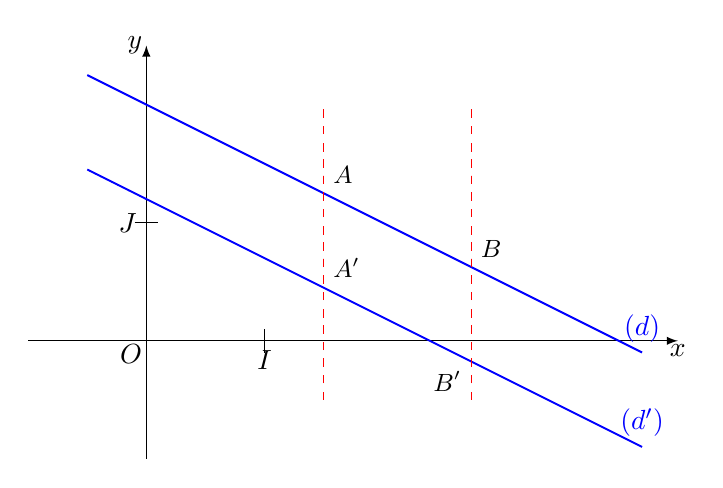
\begin{tikzpicture}[>=latex,scale=1.5]
        \draw[->] (-1,0) -- (4.5,0) node[below=-2pt] {$x$};
        \draw[->] (0,-1) -- (0,2.5) node[left=-2pt] {$y$};
        \coordinate (O) at (0,0); \draw (O) node[below left = -2pt] {$O$};
        \coordinate (I) at (1,0); \draw (I) node[below] {$I$}; \draw (1,-0.1)--(1,0.1);
        \coordinate (J) at (0,1); \draw (J) node[left] {$J$}; \draw (-0.1,1)--(0.1,1);
        \draw[color=blue,line width=0.7pt] plot[domain=-0.5:4.2,samples=200] (\x,{-0.5*\x+2}) node[above] {$(d)$};
        \draw[color=blue,line width=0.7pt] plot[domain=-0.5:4.2,samples=200] (\x,{-0.5*\x+1.2}) node[above] {$(d')$};
        \draw[color=red,dashed] plot[domain=-0.5:2,samples=200] (1.5,\x);
        \draw[color=red,dashed] plot[domain=-0.5:2,samples=200] (2.75,\x);
        \draw (1.5,1.25) node[above right] {\small$A$}; \draw (2.75,0.625) node[above right] {\small$B$};
        \draw (1.5,0.45) node[above right] {\small$A'$}; \draw (2.75,-0.175) node[below left] {\small$B'$};
    \end{tikzpicture}
\end{center}

\renewcommand\arraystretch{1.75}
\begin{tabular}{ll}
    & $(d)$ et $(d')$ sont parallèles \\
    $\Leftrightarrow$ & $ABB'A'$ est un parallélogramme \\
    $\Leftrightarrow$ & $[AB']$ et $[A'B]$ ont le même milieu \\
    $\Leftrightarrow$ & $\left\{\begin{array}{rcl} \frac{x_A + x_{B'}}{2} = \frac{x_{A'} + x_{B}}{2} \\[7pt] \frac{y_A + y_{B'}}{2} = \frac{y_{A'} + y_{B}}{2} \end{array}\right.$ \\
    $\Leftrightarrow$ & $\left\{\begin{array}{rcl} x_A + x_{B'} = x_{A'} + x_{B} \\ y_A + y_{B'} = y_{A'} + y_{B} \end{array}\right.$ \\
    $\Leftrightarrow$ & $\left\{\begin{array}{rcl} x_A - x_{B} = x_{A'} - x_{B'} \\ y_A - y_{B} = y_{A'} - y_{B'} \end{array}\right.$ \\
    $\Leftrightarrow$ & $\frac{y_B - y_A}{x_B - x_A} = \frac{y_{B'} - y_{A'}}{x_{B' }- x_{A'}}$\qquad (équivalence car $x_A = x_{A'}$ et $x_B = x_B'$)\\
    $\Leftrightarrow$ & $m = m'$
\end{tabular}
\renewcommand\arraystretch{1}

On a bien démontré que $(d) /\!/ (d') \quad \Leftrightarrow \quad m = m'$.
\end{Demo}

\begin{Exemple}
    Donner les équations réduites des droites suivantes et déterminer celles qui sont parallèles :
    \[(d_1) : y - 2x + 1 = 0 \qq (d_2) : y + 3x - 2 = 0 \qq (d_3) : 4y + 12x - 20 = 0 \qq (d_4) : y + 1 = 2x.\]
\end{Exemple}

\subsection{Droites sécantes}
Soient $(d)$ d'équation $y = mx + p$ et $(d')$ d'équation $y = m'x + p'$. D'après la propriété précédente, deux droites sont sécantes lorsque $m \neq m'$.
Dans ce cas, il existe un point d'intersection $A$ et les coordonnées de $A$ vérifient les équations des deux droites en même temps. On a donc le système suivant dont le couple $(x \pv y)$ est l'inconnue qui correspond aux coordonnées du point $A$ :
\[\left\{\begin{array}{l} y = mx + p \\y = m'x + p' \end{array}\right.\]

\begin{Exemple}
Déterminer les coordonnées du point d'intersection des droites suivantes :
\[(\Delta_1) : y = -2x + 3 \qq (\Delta_2) : y = \frac 13 x - 1\]
\end{Exemple}

\subsection{Alignement de points}

\begin{Prop}
    On considère trois points $A$, $B$ et $C$.
    \begin{enumerate}
        \item Si les trois points ont la même abscisse $k$, alors ils sont alignés.
        \item Sinon, les points sont alignés si et seulement si $(AB)$ et $(AC)$ ont le même \coef directeur.
    \end{enumerate}
\end{Prop}

\begin{Demo}
    Dans le premier cas, les points appartiennent à la même droite d'équation $x = k$ donc ils sont alignés.\par
    Dans le second cas, dire que $(AB)$ et $(AC)$ ont le même \coef directeur est équivalent à dire que ces droites sont parallèles ce qui est équivalent à dire qu'elles sont confondues (puisqu'elles ont un point commun) ce qui équivaut à dire qu'il s'agit de la même droite et donc $A$, $B$ et $C$ sont alignés.
\end{Demo}

\begin{Exemple}
    Dans chacun des cas, les points $A$, $B$ et $C$ sont-ils alignés ?
    \[A(6 \pv 0) \qq B(0 \pv 4) \qq C(3 \pv 2)\]\[A(1 \pv 3) \qq B(2 \pv 9) \qq C(4 \pv 10)\]
\end{Exemple}
\end{document}

%------ Chapitre 05
    \documentclass[10pt,openright,twoside,french]{book}

\input philippe2013
\input philippe2013_cours
\input philippe2013_sections
\input philippe2013_chapitre

\setcounter{chapter}{4}
\begin{document}

\renewcommand\PartProgramme{Fonctions}
\chapter[Variations de fonctions]{Variations de \\ fonctions}\label{ch_variations_fonctions}

\section{\'Etude graphique}

On considère une fonction $f$ définie sur un ensemble $\calig D_f$ ainsi qu'un intervalle $I$ inclus dans $\calig D_f$.\par\medskip

Dire que la fonction $f$ est croissante sur $I$ signifie que lorsque la valeur de la variable augmente sur $I$ alors l'image augmente également. Graphiquement, la courbe représentative de $f$ \og~monte~\fg.

\begin{Defi}
    Une fonction $f$ est dite \iptb{croissante}\index{fonction!croissante} sur un intervalle $I$ lorsque, \textbf{pour tous} les réels $x_1$ et $x_2$ :
    \[x_1 < x_2 \Rightarrow f(x_1) \leq f(x_2).\]
    Autrement dit, deux nombres et leur image sont classés dans le \textbf{même} ordre.
\end{Defi}

\begin{Exemple}
Fonction croissante sur l'intervalle $\intervalleff{-1,5}{4}$.
\end{Exemple}

\begin{center}
    \begin{tikzpicture}[>=latex,scale=0.9]
    \begin{scope}[xshift=1cm]
        \draw[->] (-2,0) -- (4.5,0) node[below=-2pt] {$x$};
        \draw[->] (0,-1) -- (0,2.5) node[left=-2pt] {$y$};
        \coordinate (O) at (0,0); \draw (O) node[below left = -2pt] {$O$};
        \coordinate (I) at (1,0); \draw (I) node[below] {$I$}; \draw (1,-0.1)--(1,0.1);
        \coordinate (J) at (0,1); \draw (J) node[left] {$J$}; \draw (-0.1,1)--(0.1,1);
        \draw[color=blue,line width=0.7pt] plot[domain=-1.5:4,samples=200] (\x,{ln(\x + 2)});
        \draw[red,dashed] (-1.5,0) node {$\bullet$} node[above] {\scriptsize $-1,5$}--(-1.5,{ln(0.5)}) -- (0,-0.7)node {$\bullet$} node[right] {\scriptsize $-0,7$};
        \draw[red,dashed] (4,0) node {$\bullet$} node[below] {\scriptsize $4$}--(4,{ln(6)}) -- (0,1.8)node {$\bullet$} node[left] {\scriptsize $1,8$};
    \end{scope}
    \begin{scope}[xshift=-4cm,yshift=-1.7cm]
        \tkzTabInit[nocadre]{$x$/0.75,Variation de \\ $f(x)$/1.5}{$-1{,}5$,$4$}
        \tkzTabVar{-/$-0{,}7$,+/$1{,}8$}
        \draw (3,-2.6) node {Tableau de variations};
    \end{scope}
    \begin{scope}[xshift=3cm,yshift=-1.7cm]
        \tkzTabInit[nocadre]{$x$/0.75,Signe de \\ $f(x)$/1.5}{$-1{,}5$,$-1$,$4$}
        \tkzTabLine{,-,z,+}
        \draw (5,-2.6) node {Tableau de signes};
    \end{scope}
    \end{tikzpicture}
\end{center}

\begin{Rmq}
    Lorsque $x_1 < x_2 \Rightarrow f(x_1) < f(x_2)$, on dit que la fonction est \textbf{strictement} croissante.
\end{Rmq}

Dire que la fonction $f$ est décroissante sur $I$ signifie que lorsque la valeur de la variable augmente sur $I$ alors l'image diminue. Graphiquement, la courbe représentative de $f$ \og~descend~\fg.

\begin{Defi}
    Une fonction $f$ est dite \iptb{décroissante}\index{fonction!décroissante} sur un intervalle $I$ lorsque, \textbf{pour tous} les réels $x_1$ et $x_2$ :
    \[x_1 < x_2 \Rightarrow f(x_1) \geq f(x_2).\]
    Autrement dit, deux nombres et leur image sont classés dans un ordre \textbf{contraire}.
\end{Defi}

\begin{Rmq}
    Lorsque $x_1 < x_2 \Rightarrow f(x_1) > f(x_2)$, on dit que la fonction est \textbf{strictement} décroissante.
\end{Rmq}\clearpage

\begin{Exemple}
Fonction décroissante sur l'intervalle $\intervalleff{-2}{4}$.
\end{Exemple}

\begin{center}
    \begin{tikzpicture}[>=latex,scale=0.9]
    \begin{scope}[xshift=1cm]
        \draw[->] (-2,0) -- (4.5,0) node[below=-2pt] {$x$};
        \draw[->] (0,-1) -- (0,2.5) node[left=-2pt] {$y$};
        \coordinate (O) at (0,0); \draw (O) node[below left = -2pt] {$O$};
        \coordinate (I) at (1,0); \draw (I) node[below] {$I$}; \draw (1,-0.1)--(1,0.1);
        \coordinate (J) at (0,1); \draw (J) node[left] {$J$}; \draw (-0.1,1)--(0.1,1);
        \draw[color=blue,line width=0.7pt] plot[domain=-2:4,samples=200] (\x,{1/(\x+2.4)-1});
        \draw[red,dashed] (-2,0) node {$\bullet$} node[below] {\scriptsize $-2$}--(-2,{1/0.4-1}) -- (0,1.5)node {$\bullet$} node[right] {\scriptsize $1,5$};
        \draw[red,dashed] (4,0) node {$\bullet$} node[above] {\scriptsize $4$}--(4,{1/6.4-1}) -- (0,{1/6.4-1})node {$\bullet$} node[left] {\scriptsize $-0,8$};
    \end{scope}
    \begin{scope}[xshift=-4cm,yshift=-1.7cm]
        \tkzTabInit[nocadre]{$x$/0.75,Variation de \\ $f(x)$/1.5}{$-2$,$4$}
        \tkzTabVar{+/$1{,}5$,-/$-0{,}8$}
        \draw (3,-2.6) node {Tableau de variations};
    \end{scope}
    \begin{scope}[xshift=3cm,yshift=-1.7cm]
        \tkzTabInit[nocadre]{$x$/0.75,Signe de \\ $f(x)$/1.5}{$-2$,$-1{,}4$,$4$}
        \tkzTabLine{,+,z,-}
        \draw (5,-2.6) node {Tableau de signes};
    \end{scope}
    \end{tikzpicture}
\end{center}

\begin{Rmq}
    Sur tout son ensemble de définition, les variations d'une fonction $f$ peuvent changer.
\end{Rmq}

\begin{Exemple}
Fonction définie sur l'intervalle $\intervalleff{-4}{3}$.
\end{Exemple}

\begin{center}
    \begin{tikzpicture}[>=latex,scale=0.9]
    \begin{scope}[xshift=1cm]
        \draw[help lines] (-4.2,-2.5) grid (3.5,3.5);
        \draw[->] (-4.2,0) -- (3.5,0) node[below=-2pt] {$x$};
        \draw[->] (0,-2.5) -- (0,3.5) node[left=-2pt] {$y$};
        \coordinate (O) at (0,0); \draw (O) node[below left = -2pt] {$O$};
        \coordinate (I) at (1,0); \draw (I) node[below] {$I$}; \draw (1,-0.1)--(1,0.1);
        \coordinate (J) at (0,1); \draw (J) node[left] {$J$}; \draw (-0.1,1)--(0.1,1);
        \draw[color=blue,line width=0.7pt] plot[domain=-4:3,samples=200] (\x,{(\x+3.5)*(\x+1)*(\x-2)/10});
    \end{scope}
    \begin{scope}[xshift=-5cm,yshift=-2.5cm]
        \tkzTabInit[nocadre,espcl=2]{$x$/0.75,Variation de \\ $f(x)$/1.5}{$4$,,,$3$}
        \tkzTabVar{-/,+/,-/,+/}
        \draw (5,-2.6) node {Tableau de variations};
    \end{scope}
    \begin{scope}[xshift=5cm,yshift=-2.5cm]
        \tkzTabInit[nocadre,espcl=1]{$x$/0.75,Signe de \\ $f(x)$/1.5}{$4$,{$-3,5$},$-1$,$2$,$3$}
        \tkzTabLine{,-,z,+,z,-,z,+}
        \draw (5,-2.6) node {Tableau de signes};
    \end{scope}
    \end{tikzpicture}
\end{center}

\begin{Exemple}
    On donne les variations et le signe d'une fonction $f$ définie sur l'intervalle $\intervalleff{-3}{4}$. Dessiner une représentation graphique qui pourrait correspondre à ce tableau :
    \begin{center}
        \begin{tikzpicture}
            \tkzTabInit[nocadre,espcl=2]{$x$/0.75,Variations de \\ $f(x)$/1.5,Signes de \\ $f(x)$/1.5}{$-3$,{$-2,5$},$-1$,{$-0,25$},$1$,$4$}
            \tkzTabVar{+/$2$,R,-/$-2$,R,+/$3$,-/$1$}
            \tkzTabLine{,+,z,,-,,z,,+}
        \end{tikzpicture}
    \end{center}
\end{Exemple}

\section{Extremum}
Graphiquement, les extrema sont les points les plus hauts d'une courbe ou les plus bas. Ce sont ceux dont l'\textbf{ordonnée} est donc la plus grande ou la plus petite. On s'intéresse dans ce cas aux images par la fonction représentée.\medskip

\begin{Defi}
    On dit que $f$ admet un \ipt{maximum} en $a$ sur $\calig D_f$ lorsque, pour tout réel $x \in \calig D_f$, $f(x) \leq f(a)$.\par
    On dit que $f$ admet un \ipt{minimum} en $b$ sur $\calig D_f$ lorsque, pour tout réel $x \in \calig D_f$, $f(x) \geq f(a)$.
\end{Defi}

\begin{Exemple}

Sur la figure ci-dessous, on a $\min_{\calig D_f} f = 0$ et $\max_{\calig D_f} f \approx 4,8$.\par
Autrement dit, pour tout $x \in \calig D_f$, $f(x) \geq 0$ et $f(x) \leq 4,8$.

\begin{center}
    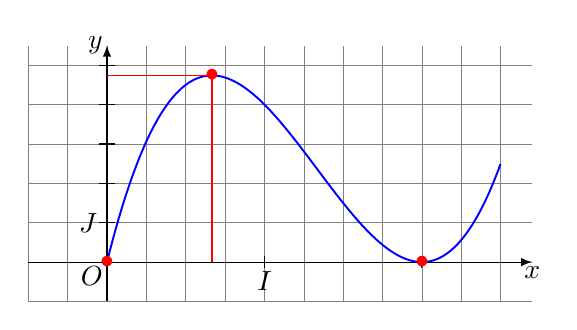
\begin{tikzpicture}[>=latex,xscale=2,yscale=0.5]
    \draw[help lines] (-0.5,-1) grid[xstep=0.25] (2.7,5.5);
        \draw[->] (-0.5,0) -- (2.7,0) node[below=-2pt] {$x$};
        \draw[->] (0,-1) -- (0,5.5) node[left=-2pt] {$y$};
        \coordinate (O) at (0,0); \draw (O) node[below left = -2pt] {$O$};
        \coordinate (I) at (1,0); \draw (I) node[below] {$I$}; \foreach \x in {1,2}  \draw (\x,-0.15)--(\x,0.15);
        \coordinate (J) at (0,1); \draw (J) node[left] {$J$}; \foreach \x in {1,...,5} \draw (-0.05,\x)--(0.05,\x);
        \draw[color=blue,line width=0.7pt] plot[domain=0:2.5,samples=200] (\x,{\x*(4-2*\x)^2});
        \draw[red] (O) node {$\bullet$};
        \draw[red] (2,0) node {$\bullet$};
        \draw[red] (2/3,0) -- (2/3,2*64/27) node {$\bullet$} -- (0,2*64/27);
    \end{tikzpicture}
\end{center}

On remarque que le minimum est atteint deux fois : pour $x = 0$ et pour $x = 2$.
\end{Exemple}

\section{Résolution graphique d'une inéquation}
On appelle $\calig C_f$ et $\calig C_g$ les représentations graphiques des fonctions $f$ et $g$.

\subsection{Inéquation du type $f(x) < k$}
\begin{Prop}
    Soit $k \in \R$. Les solutions de l'inéquation $f(x) < k$ sont les \iptb{abscisses} des points de la courbe $\calig C_f$ situés au-dessous de la droite d'équation $y = k$.
\end{Prop}

\begin{Exemple}
Soit $\calig D_f = \intervalleff{-3}{3}$. Donner l'ensemble des solutions des équations $f(x) < 4$ puis $f(x) \geq 4$.

\begin{center}
    \begin{tikzpicture}[>=latex,scale=0.5]
    \draw[help lines] (-3.5,-1) grid (3.5,10.5);
        \draw[->] (-3.5,0) -- (3.5,0) node[below=-2pt] {$x$};
        \draw[->] (0,-1) -- (0,10.5) node[left=-2pt] {$y$};
        \coordinate (O) at (0,0); \draw (O) node[below left = -2pt] {$O$};
        \coordinate (I) at (1,0); \draw (I) node[below] {$I$}; \foreach \x in {-3,...,3}  \draw (\x,-0.1)--(\x,0.1);
        \coordinate (J) at (0,1); \draw (J) node[left] {$J$}; \foreach \x in {-1,...,10} \draw (-0.1,\x)--(0.1,\x);
        \draw[color=blue,line width=0.7pt,name path=Parabole] plot[domain=-3:3,samples=200] (\x,\x*\x) node[right] {$\calig C_f$};
        \draw[red,name path = Droite] (-3.5,4) -- (3.5,4) node[above right] {y = 4};
        \path [name intersections={of = Parabole and Droite}];
        \coordinate (A) at (intersection-1);
        \draw[red,dashed] let\p1=($(A)$) in (\p1) node {$\bullet$}--(\x1,0);
        \coordinate (B) at (intersection-2);
        \draw[red,dashed] let\p1=($(B)$) in (\p1) node {$\bullet$}--(\x1,0);
        \draw (-8,10) node {$f(x) < 4 \Leftrightarrow x \in \intervalleoo{-2}{2}$.};
        \draw (-8,9) node {$f(x) \geq 4 \Leftrightarrow x \in \intervalleff{-3}{-2} \cup \intervalleff{2}{3}$.};
    \end{tikzpicture}
\end{center}
\end{Exemple}


\subsection{Inéquation du type $f(x) < g(x)$}
\begin{Prop}
    Les solutions de l'inéquation $f(x) < g(x)$ sont les \iptb{abscisses} des points de la courbe $\calig C_f$ situés au-dessous de la courbe $\calig C_g$.
\end{Prop}\clearpage

\begin{Exemple}
On considère deux fonctions $f$ et $g$ définies sur $\intervalleff{-3}{3}$ dont voici les représentations graphiques :

\begin{center}
    \begin{tikzpicture}[>=latex]
    \draw[help lines] (-3.5,-2.5) grid (3.5,3.5);
        \draw[->] (-3.5,0) -- (3.5,0) node[below=-2pt] {$x$};
        \draw[->] (0,-2.5) -- (0,3.5) node[left=-2pt] {$y$};
        \coordinate (O) at (0,0); \draw (O) node[below left = -2pt] {$O$};
        \coordinate (I) at (1,0); \draw (I) node[below] {$I$}; \foreach \x in {-3,...,3}  \draw (\x,-0.1)--(\x,0.1);
        \coordinate (J) at (0,1); \draw (J) node[above left] {$J$}; \foreach \x in {-2,...,3} \draw (-0.1,\x)--(0.1,\x);
        \draw[color=blue,line width=0.7pt,name path=ParaboleA] plot[domain=-3:3,samples=200] (\x,{((\x)^2+2*\x-3)/5}) node[right] {$\calig C_f$};
        \draw[color=red,line width=0.7pt,name path=ParaboleB] plot[domain=-3:3,samples=200] (\x,{(-(\x-1)^2+6)/5}) node[right] {$\calig C_g$};
        \path [name intersections={of = ParaboleA and ParaboleB}];
        \coordinate (A) at (intersection-1);
        \draw[color=OliveGreen,dashed] let\p1=($(A)$) in (\p1) node {$\bullet$}--(\x1,0);
        \coordinate (B) at (intersection-2);
        \draw[color=OliveGreen,dashed] let\p1=($(B)$) in (\p1) node {$\bullet$}--(\x1,0);
    \end{tikzpicture}
\end{center}

Ici, $f(x) \leq g(x) \Leftrightarrow x \in \intervalleff{-2}{2}$ et $f(x) > g(x) \Leftrightarrow x \in \intervallefo{-3}{-2} \cup \intervalleof{2}{3}$.
\end{Exemple}

\end{document}

%------ Chapitre 06
    \input{2nde_06_Fonctions_Affines/2nde_06_Fonctions_Affines.tex}

%------ Index
\setcounter{tocdepth}{1}

\renewenvironment{theindex}
{\cleardoublepage
{\color{midblue}
       \vspace*{10\p@}%
        \begin{minipage}[c]{\textwidth}
        \rule{\textwidth}{1ex}
        \par\nobreak
        \begin{flushright}
            \Huge\bfseries Index \\ des notions définies
         \end{flushright}
        \par\nobreak
        \rule{\textwidth}{1ex}
         \end{minipage}
    \vskip 40\p@
}
\renewcommand{\item}{\par\hangindent 40pt}
\begin{multicols}{2}
}
{\end{multicols}}


\entete{}{}{}
\printindex\addcontentsline{toc}{chapter}{\protect Index des notions définies}

\vspace{\stretch{1}}

\[***\]

\begin{center}
\'Ecrit par Philippe \bsc{De Sousa}.\par
Dernière modification le \today.
\end{center}

\end{document} 